\documentclass[11pt,a4paper]{article}

\usepackage[T1]{fontenc}
\usepackage[utf8]{inputenc}
\usepackage{lmodern}
\usepackage[margin=1in]{geometry}
\usepackage{amsmath,amssymb,amsthm,mathtools}
\usepackage{booktabs}
\usepackage{array}
\usepackage{tabularx}
\usepackage{float}
\usepackage[hidelinks]{hyperref}
\usepackage[nameinlink,noabbrev]{cleveref}
\usepackage{microtype}
\usepackage{enumitem}
\usepackage{siunitx}
\usepackage{xcolor}
\usepackage{tcolorbox}
\tcbuselibrary{skins,breakable}
\usepackage{thmtools}
\usepackage{tikz}
\usetikzlibrary{arrows.meta,positioning,calc,fit,backgrounds,matrix,decorations.pathmorphing}
\usepackage{pgfplots}
\pgfplotsset{compat=1.18}
\usepackage{longtable}
\usepackage{multirow}
\usepackage{makecell}
\usepackage{bm}
\usepackage{csquotes}

\sisetup{
    detect-all,
    round-mode = figures,
    round-precision = 10,
    exponent-mode = input,
    exponent-product = \times,
    group-separator = {\,},
    group-minimum-digits = 4
}

\newtheorem{theorem}{Theorem}[section]
\newtheorem{corollary}[theorem]{Corollary}
\newtheorem{lemma}[theorem]{Lemma}
\theoremstyle{definition}
\newtheorem{definition}[theorem]{Definition}
\newtheorem{conjecture}[theorem]{Conjecture}
\newtheorem{proposition}[theorem]{Proposition}
\newtheorem{assumption}[theorem]{Assumption}
\newtheorem{principle}[theorem]{Principle}
\newtheorem{construction}[theorem]{Construction}
\newtheorem{claim}[theorem]{Claim}
\newtheorem{conditionalstep}[theorem]{Conditional Step}
\theoremstyle{remark}
\newtheorem*{remark}{Remark}

\makeatletter
\def\theHtheorem{\thesection.\thetheorem}
\def\theHcorollary{\theHtheorem}
\def\theHlemma{\theHtheorem}
\def\theHdefinition{\theHtheorem}
\def\theHconjecture{\theHtheorem}
\def\theHproposition{\theHtheorem}
\def\theHassumption{\theHtheorem}
\def\theHprinciple{\theHtheorem}
\def\theHconstruction{\theHtheorem}
\def\theHclaim{\theHtheorem}
\def\theHconditionalstep{\theHtheorem}
\makeatother

\DeclareMathOperator{\tr}{Tr}
\DeclareMathOperator{\rank}{rank}
\DeclareMathOperator{\SF}{SF}
\DeclareMathOperator{\Ind}{Ind}
\DeclareMathOperator{\argmin}{arg\,min}

\newcolumntype{Y}{>{\raggedright\arraybackslash}X}

\newcommand{\Seam}{\Sigma}
\newcommand{\inv}{\iota}
\newcommand{\Mpl}{\bar M_{\mathrm{Pl}}}
\newcommand{\Mplunred}{M_{\mathrm{Pl}}}
\newcommand{\cthree}{c_3}
\newcommand{\atheta}{a_\theta}
\newcommand{\phibase}{\varphi_{\mathrm{base}}}
\newcommand{\phiz}{\varphi_0}
\newcommand{\deltatop}{\delta_{\mathrm{top}}}
\newcommand{\bone}{b_1}
\newcommand{\SM}{\mathrm{SM}}
\newcommand{\QCD}{\mathrm{QCD}}
\newcommand{\Oadm}{\Omega_{\mathrm{adm}}}
\newcommand{\Cmin}{\mathcal C_{\min}}
\newcommand{\Ageom}{\mathcal A_{\mathrm{geom}}}
\newcommand{\Atrans}{\mathcal A_{\mathrm{trans}}}
\newcommand{\Arec}{\mathcal A_{\mathrm{rec}}}
\newcommand{\Aobs}{\mathcal A_{\mathrm{obs}}}
\newcommand{\Vadm}{\mathcal V_{\mathrm{adm}}}
\newcommand{\Hrel}{\mathcal H_{\mathrm{rel}}}
\newcommand{\Hhub}{H_{\mathrm{hub}}}
\newcommand{\Htot}{\mathcal H_{\mathrm{tot}}}
\newcommand{\Gammaeff}{\Gamma_{\mathrm{eff}}}
\newcommand{\lambdaY}{\lambda_Y}
\newcommand{\Pred}{\operatorname{Pred}}
\newcommand{\gcar}{g_{\mathrm{car}}}
\newcommand{\Dstart}{D_{\mathrm{start}}}
\newcommand{\Tcore}{\mathfrak T_{\mathrm{core}}}
\newcommand{\Tbridge}{\mathfrak T_{\mathrm{bridge}}}
\newcommand{\Tker}{\mathfrak T_{\mathrm{ker}}}
\newcommand{\Tcomp}{\mathfrak T_{\mathrm{comp}}}

\title{%
    \textbf{TFPT: Carrier Algebra, Compression Identities, and Finite Completion}\\[0.5em]
    \Large An overdetermined rank-5 spectral theory on the oriented double cover
}
\author{Stefan Hamann \and Alessandro Rizzo}
\date{\textbf{INTERNAL DRAFT -- \today}}

\begin{document}
\maketitle

\begin{abstract}
A minimal carrier $E_3\oplus E_2$ on the oriented double cover is shown to be the unique rank-5 split satisfying $\dim\Lambda^{\mathrm{even}}E=16$ and $\tr_EY^2=5/6$. This carrier already forces the global Standard Model group $S(U(3)\times U(2))\cong(SU(3)\times SU(2)\times U(1)_Y)/\mathbb Z_6$, one chiral family with $\nu^c$ from the positive half-spinor, the hypercharge--seam inversion $6Y^2-Y-\mathbf 1=0$, and a self-consistent electromagnetic closure equation whose positive root gives $\alpha^{-1}(0)=\num{137.0360}$.

On the canonical branch the carrier packet is overdetermined by a set of compression identities: the rank-lock $2^{g-3}=g-1$ has the unique integral solution $g=5$; the $41$-chain $48\,I_1^{\mathrm{EW}}=32\,k_{\mathrm{EW}}=10\,b_1=\Omega_{\mathrm{adm}}\gamma+1=41$ collapses four algebraic layers onto one integer; and the Cabibbo inversion $\varphi_0=\frac12(1-\sqrt{1-4\lambda_C^2})$ compresses the bridge outputs $(\beta,\Omega_b,\lambda_C,\sin^2\theta_{13})$ into a single seed. Wrong discrete worlds fail the electromagnetic closure categorically: two families give $\alpha^{-1}\approx 156$, four families give $\alpha^{-1}\approx 125$, and two Higgs doublets give $\alpha^{-1}\approx 136$.

The remaining open problem is a finite completion program with five explicit interfaces: a family local-system theorem hardening the flavor lift and the occupancy interpretation of $\Omega_{\mathrm{adm}}=48$, a bosonic relative index selecting the unique light Higgs doublet, a $\chi$-channel heat-kernel closure generating $\bar M_{\mathrm{Pl}}$ and the electroweak vacuum from one geometric response, a discrete hexagonal transport kernel for Yukawas, mixings, confinement, and strong CP, and a comparison bridge fixing scheme and threshold conventions. E$_8$ is retained only as downstream scale grammar; record algebra, horizons, and prediction semantics are conditional appendix material. Benchmark tables, a falsification matrix, and finite proof obligations separate hard results from bridges and completion targets throughout.
\end{abstract}

\begin{tcolorbox}[colback=gray!5, colframe=gray!60, breakable,
    title={\textbf{Reading Status for the Present Paper}}, fonttitle=\bfseries]
\begin{itemize}[leftmargin=1.5em, topsep=3pt, itemsep=3pt]
    \item \textbf{Hard:} oriented double cover, seam $\Seam$, involution $\inv$, minimal carrier $E_3\oplus E_2$, global group $S(U(3)\times U(2))\cong \frac{SU(3)\times SU(2)\times U(1)_Y}{\mathbb Z_6}$, one chiral family, carrier norm $5/6$, the abelian-index formula, and the established kernel numerics $(\cthree,\deltatop,\phiz,\alpha)$.
    \item \textbf{Bridge:} family space $F$, occupancy $\Oadm=48$, the occupancy reinterpretation $\deltatop=\Oadm\cthree^4$, the comparison map $\mathcal R_{\SM}$, and the benchmark interface from kernel outputs to observables.
    \item \textbf{Completion:} bosonic relative index for Higgs selection, $\chi$-channel heat-kernel closure, regularized Yukawa kernels and path-length masses, confinement as admissible word selection, and strong-CP cancellation.
    \item \textbf{Conditional:} downstream E$_8$ scale grammar, record algebra, horizons, prediction semantics, and the final compiler theorem.
\end{itemize}
\end{tcolorbox}

\tableofcontents

\section{Reading guide and claim map}

The paper is organized in three reading layers:
\begin{itemize}[leftmargin=1.5em, topsep=3pt, itemsep=2pt]
    \item \textbf{Big picture:} one section explains what TFPT claims in plain language before the detailed datum and conventions begin.
    \item \textbf{Detail:} the main body then runs from primitive core and hard carrier kernel through kernel numerics, the two completion programs, the particle/mass compiler, and the benchmark interface.
    \item \textbf{Proof sketches:} the main text gives only the central proof sketches, while dense technical derivations remain in appendices or companion material.
\end{itemize}
The status language is also fixed once and for all:
\begin{itemize}[leftmargin=1.5em, topsep=3pt, itemsep=2pt]
    \item \textbf{Hard} means established carrier or kernel structure.
    \item \textbf{Bridge} means a structural lift or comparison interface that organizes the compiler but is not yet a closed theorem.
    \item \textbf{Completion} means a theorem-sized open interface that would close a genuine physics sector.
    \item \textbf{Conditional} means a downstream or appendix-level statement that is only accepted once the completion layer is granted.
\end{itemize}

\begin{figure}[t]
\centering
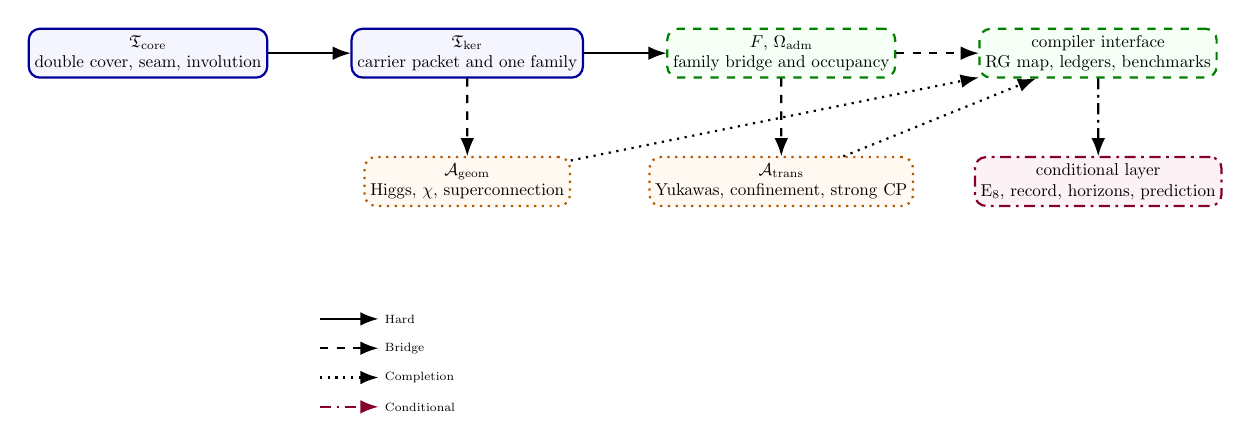
\begin{tikzpicture}[
    scale=0.62,
    transform shape,
    >=Latex,
    node distance=1.6cm and 1.7cm,
    hard/.style={draw=blue!60!black, thick, rounded corners, fill=blue!4, align=center, minimum width=2.8cm, minimum height=1cm},
    bridge/.style={draw=green!50!black, dashed, thick, rounded corners, fill=green!4, align=center, minimum width=2.9cm, minimum height=1cm},
    completion/.style={draw=orange!70!black, dotted, thick, rounded corners, fill=orange!5, align=center, minimum width=3.0cm, minimum height=1cm},
    conditional/.style={draw=purple!70!black, dash pattern=on 4pt off 2pt on 1pt off 2pt, thick, rounded corners, fill=purple!5, align=center, minimum width=3.0cm, minimum height=1cm}
]
\node[hard] (core) {$\Tcore$\\double cover, seam, involution};
\node[hard, right=of core] (carrier) {$\Tker$\\carrier packet and one family};
\node[bridge, right=of carrier] (bridge) {$F$, $\Oadm$\\family bridge and occupancy};
\node[completion, below=of carrier] (geom) {$\Ageom$\\Higgs, $\chi$, superconnection};
\node[completion, below=of bridge] (trans) {$\Atrans$\\Yukawas, confinement, strong CP};
\node[bridge, right=of bridge] (cmp) {compiler interface\\RG map, ledgers, benchmarks};
\node[conditional, below=of cmp] (cond) {conditional layer\\E$_8$, record, horizons, prediction};
\draw[->, thick] (core) -- (carrier);
\draw[->, thick] (carrier) -- (bridge);
\draw[->, dashed, thick] (carrier) -- (geom);
\draw[->, dashed, thick] (bridge) -- (trans);
\draw[->, dashed, thick] (bridge) -- (cmp);
\draw[->, dotted, thick] (geom) -- (cmp);
\draw[->, dotted, thick] (trans) -- (cmp);
\draw[->, dash pattern=on 4pt off 2pt on 1pt off 2pt, thick] (cmp) -- (cond);
\coordinate (legone) at ($(geom.south west)+(-0.9,-2.3)$);
\draw[->, thick] (legone) -- ++(1.2,0) node[right, black, font=\scriptsize] {Hard};
\coordinate (legtwo) at ($(legone)+(0,-0.6)$);
\draw[->, dashed, thick] (legtwo) -- ++(1.2,0) node[right, black, font=\scriptsize] {Bridge};
\coordinate (legthree) at ($(legtwo)+(0,-0.6)$);
\draw[->, dotted, thick] (legthree) -- ++(1.2,0) node[right, black, font=\scriptsize] {Completion};
\coordinate (legfour) at ($(legthree)+(0,-0.6)$);
\draw[->, dash pattern=on 4pt off 2pt on 1pt off 2pt, thick, purple!70!black] (legfour) -- ++(1.2,0) node[right, black, font=\scriptsize] {Conditional};
\end{tikzpicture}
\caption{Claim map for the carrier-first compiler form. Hard fixes the carrier and numerical kernel, Bridge organizes family lift and comparison, Completion closes geometry and transport, and Conditional collects downstream extensions.}
\label{fig:dependency-map}
\end{figure}

\begin{table}[t]
\centering
\scriptsize
\begin{tabularx}{\linewidth}{@{}>{\raggedright\arraybackslash}p{0.23\linewidth}>{\raggedright\arraybackslash}p{0.12\linewidth}YY@{}}
\toprule
Layer or statement & Status & Proof source or missing lemma & Main empirical or structural test \\
\midrule
Oriented double cover, seam, involution & Hard & starting geometric datum; fixed throughout the paper & structural consistency of all later layers \\
Minimal carrier $E_3\oplus E_2$ & Hard & proof sketch given in \Cref{sec:minimal-carrier-proof} & failure would collapse the whole packet \\
One-family packet $S^+=\Lambda^{\mathrm{even}}E$ & Hard & decomposition and proof sketch given in the main text & group/matter mismatch would be global \\
Kernel numerics $(\cthree,\deltatop,\phiz,\alpha)$ & Hard & carrier-form closure equations summarized in the main text & scheme discipline for observable comparison \\
Family count $N_{\mathrm{fam}}=3$ from patch deficit & Hard & patch-deficit route and proof sketch given & family-count interpretation \\
Family space $F$ for flavor splitting & Bridge & monodromy for nondegeneracy and mixing still open & flavor phases, CKM / PMNS \\
Occupancy $\Oadm=48$ and $\deltatop=\Oadm\cthree^4$ & Bridge & immediate count corollary; occupancy reinterpretation is bridge & topological surcharge \\
Comparison map $\mathcal R_{\SM}$ & Bridge & declared RG / threshold bookkeeping & convention-complete theory-versus-data translation \\
Bosonic relative index selecting $\Phi$ & Completion & missing bosonic index closure & unique light doublet / doublet-triplet split \\
$\chi$-channel Einstein bridge & Completion & missing relative heat-kernel closure & one closure for $\Mpl$, $v$, and the scale map \\
Regularized Yukawa kernel closure & Completion & missing phase-distance theorem & $m_f$, $\lambda_C$, $\theta_{13}$, CKM / PMNS sharpenings \\
Confinement and strong CP closure & Completion & missing bound-state control and positivity hardening & hadron spectrum and $\bar\theta$ null tests \\
E$_8$, record, horizons, prediction semantics & Conditional & deferred to appendices and the conditional compiler theorem & downstream extension rather than main-text hard claim \\
\bottomrule
\end{tabularx}
\caption{Status matrix for the carrier-first compiler form.}
\label{tab:status-matrix}
\end{table}

\section{Big picture: what TFPT actually claims}

TFPT is presented here as a carrier-first theory of admissible vacua on the oriented double cover. The seam involution enforces the minimal carrier $E_3\oplus E_2$. That carrier fixes the global Standard Model group, hypercharge, and one chiral family. The family count $N_{\mathrm{fam}}=3$ is then supported by two independent routes: a local patch-deficit count and a global monodromy argument. The monodromy space $F$ is retained not as the origin of the number three, but as the carrier of nondegeneracy, flavor phases, and mixing. A bosonic relative index is intended to select the Higgs, the $\chi$ channel is intended to generate both the Planck scale and the electroweak vacuum, and a discrete phase transport is intended to generate Yukawas, mixings, confinement, and strong CP. The comparison map then translates this compiler into PDG-style observables.

\begin{tcolorbox}[colback=blue!3, colframe=blue!50!black, breakable,
    title={\textbf{Carrier-first compiler chain}}, fonttitle=\bfseries]
\begin{equation}
\label{eq:compiler-chain}
\begin{aligned}
(\widetilde M\to M,\Seam,\inv,\chi)
&\Rightarrow
(E_3\oplus E_2,\ G_{\SM}^{\mathrm{glob}},\ S^+)\\
&\Rightarrow
(N_{\mathrm{fam}}=3,\ \Oadm=48,\ \Phi)\\
&\Rightarrow
(\Mpl,\ v,\ \mathcal Y_f)\\
&\Rightarrow
(m_f,\ V_{\mathrm{CKM}},\ U_{\mathrm{PMNS}},\ \text{hadrons},\ \Pred).
\end{aligned}
\end{equation}
\end{tcolorbox}

The remainder of the main text sharpens each arrow of this chain in turn.

\section{Primitive core and hard carrier kernel}

\subsection{Primitive core and conventions}

We use natural units $c=\hbar=1$. Relative operators are formulated in Euclidean signature and compared through a declared Wick-rotation bridge when Lorentzian language is needed. Higgs fields are denoted by $\Phi$, Hamiltonians by $\mathcal H$, and the cosmological Hubble rate by $\Hhub(t)$; this avoids overloading the letter $H$. Newton's constant is always $G_N$, while $G_{\SM}^{\mathrm{glob}}$ is reserved for the global Standard Model gauge quotient. The seam is denoted by $\Seam$, the involution by $\inv$, and word parity by $\varepsilon(w)$.

When color-center notation is needed later, we use multiplicative notation
\[
z(w)\in\{1,\omega,\omega^2\},
\qquad
\omega=e^{2\pi i/3}.
\]
Thus center neutrality means $z(w)=1$.

\[
\Tcore
:=
\bigl(
\widetilde M\to M,\ \Seam,\ \inv,\ D_{\mathrm{rel}},\ \mathsf{Adm}
\bigr).
\]
Here \enquote{relative} always means comparison with a declared reference operator or reference-subtracted action, and $\mathsf{Adm}$ denotes the admissibility predicate on relative sectors. The technical tables for relative objects, layered bridge/completion data, and the constants atlas are collected in Appendix~\ref{app:tech} and Appendix~\ref{app:constants}; they are kept out of the early main-text flow so that the carrier kernel appears before the technical bookkeeping apparatus.

\subsection{Minimal carrier theorem}
\label{sec:minimal-carrier-proof}

\begin{theorem}[Minimal carrier theorem]
Let $E=E_b\oplus E_s$ be a split carrier with traceless diagonal generator
\[
Y_{b,s}
=
\mathrm{diag}\!\left(
\underbrace{-\frac1b,\ldots,-\frac1b}_{b\ \text{times}},
\underbrace{\frac1s,\ldots,\frac1s}_{s\ \text{times}}
\right).
\]
If one simultaneously requires
\begin{equation}
\label{eq:minimal-carrier-conditions}
\dim \Lambda^{\mathrm{even}}E=16,
\qquad
\tr_E Y_{b,s}^2=\frac56,
\end{equation}
then necessarily $\{b,s\}=\{3,2\}$.
\end{theorem}

\begin{proof}
Write $g=b+s$. Since
\[
\dim \Lambda^{\mathrm{even}}E=2^{g-1},
\]
the first condition gives $g=5$. For the diagonal generator above one has
\[
\tr_E Y_{b,s}^2
=
b\left(\frac{1}{b^2}\right)+s\left(\frac{1}{s^2}\right)
=
\frac1b+\frac1s
=
\frac{b+s}{bs}
=
\frac{5}{bs}.
\]
Imposing $\tr_E Y_{b,s}^2=5/6$ yields $bs=6$. Together with $b+s=5$ this forces the unordered solution $\{b,s\}=\{3,2\}$.
\end{proof}

Hence from now on
\[
E=E_3\oplus E_2,
\qquad
P_3=\frac{\mathbf 1-\inv}{2},
\qquad
P_2=\frac{\mathbf 1+\inv}{2},
\]
and the hypercharge operator is read concretely as
\begin{equation}
\label{eq:explicit-hypercharge}
Y
=
\mathrm{diag}\!\left(-\frac13,-\frac13,-\frac13,\frac12,\frac12\right)
=
-\frac13 P_3+\frac12 P_2
=
\frac1{12}\mathbf 1+\frac5{12}\inv.
\end{equation}

\begin{lemma}[Hypercharge--seam inversion]
On the minimal carrier, the seam involution is recovered from hypercharge by
\begin{align}
\inv&=\frac{12Y-\mathbf 1}{5},
\label{eq:hypercharge-seam-inversion}\\
(12Y-\mathbf 1)^2&=25\,\mathbf 1,
\nonumber\\
6Y^2-Y-\mathbf 1&=0.
\label{eq:carrier-polynomial}
\end{align}
Consequently the carrier projectors are
\[
P_2=\frac{\mathbf 1+\inv}{2}=\frac{2(3Y+\mathbf 1)}{5},
\qquad
P_3=\frac{\mathbf 1-\inv}{2}=\frac{3(\mathbf 1-2Y)}{5}.
\]
\end{lemma}

\begin{proof}
The affine relation between $Y$ and $\inv$ is inverted algebraically. Squaring the result and using $\inv^2=\mathbf 1$ gives the quadratic carrier polynomial. The projector formulas then follow from $P_2=(\mathbf 1+\inv)/2$ and $P_3=(\mathbf 1-\inv)/2$.
\end{proof}

\begin{remark}[Two-point carrier algebra]
Because the minimal carrier satisfies $6Y^2-Y-\mathbf 1=0$, every analytic function of $Y$ reduces to
\[
f(Y)=A_f\,\mathbf 1+B_f\,Y,
\qquad
A_f=\frac{2f(1/2)+3f(-1/3)}{5},
\qquad
B_f=\frac{6\bigl(f(1/2)-f(-1/3)\bigr)}{5}.
\]
Thus the hard carrier is effectively a two-point algebra supported on the spectral values $-1/3$ and $1/2$, and the projectors $P_3,P_2$ are already polynomial functions of $Y$.
\end{remark}

The two carrier invariants used repeatedly below are
\[
\gamma=\tr_EY^2=\frac56,
\qquad
B=\frac{\rank E_3}{\rank E_2}=\frac32.
\]
\begin{corollary}[Carrier norm from the carrier polynomial]
The carrier polynomial already fixes
\[
\gamma=\tr_EY^2=\frac16\tr_E(Y+\mathbf 1)=\frac56,
\]
since $\tr_EY=0$ and $\rank E=5$.
\end{corollary}

\begin{corollary}[Minimal carrier compression]
On the minimal carrier branch,
\[
B\gamma=\frac32\cdot\frac56=\frac54.
\]
\end{corollary}

We package the hard kernel as
\[
\Cmin=(E_3\oplus E_2,\ Y,\ S^+,\ \gamma,\ B).
\]

\subsection{Global gauge group and one-family packet}

\begin{theorem}[Global Standard Model theorem]
The determinant-preserving connected stabilizer of the minimal carrier split is
\[
G_{\SM}^{\mathrm{glob}}
=
S(U(3)\times U(2))
\cong
\frac{SU(3)\times SU(2)\times U(1)_Y}{\mathbb Z_6}.
\]
\end{theorem}

\begin{proof}[Proof sketch]
Automorphisms preserving the split act independently on $E_3$ and $E_2$, while the determinant-one condition is imposed only on the full carrier. This gives $S(U(3)\times U(2))$. The standard covering map from $SU(3)\times SU(2)\times U(1)_Y$ to this determinant-preserving stabilizer has the canonical $\mathbb Z_6$ subgroup as kernel, yielding the stated global form.
\end{proof}

Matter is read from the positive half-spinor
\[
S^+=\Lambda^{\mathrm{even}}E,
\qquad
\dim S^+=16.
\]

\begin{theorem}[One carrier family]
The positive half-spinor of the minimal carrier decomposes as
\[
S^+
\cong
(1,1)_0\oplus(3,2)_{1/6}\oplus(\bar 3,1)_{-2/3}\oplus(\bar 3,1)_{1/3}\oplus(1,2)_{-1/2}\oplus(1,1)_1,
\]
that is, exactly one chiral Standard Model family with $\nu^c$. Equivalently, in the familiar unified packaging language,
\[
S^+\cong \mathbf 1\oplus \mathbf{10}\oplus \overline{\mathbf 5}.
\]
\end{theorem}

\begin{proof}[Proof sketch]
One has
\[
S^+=\Lambda^0E\oplus\Lambda^2E\oplus\Lambda^4E.
\]
For the minimal carrier,
\[
\Lambda^2E
\cong
\Lambda^2E_3\oplus(E_3\otimes E_2)\oplus\Lambda^2E_2.
\]
Because the full determinant is trivial in $S(U(3)\times U(2))$, the $\Lambda^4E$ sector is dual to $E$ and yields the remaining $(1,2)_{-1/2}$ and $(\bar 3,1)_{1/3}$ pieces. Hypercharges are obtained by adding the diagonal carrier charges from $Y=\mathrm{diag}(-1/3,-1/3,-1/3,1/2,1/2)$, and the multiplicities sum to $1+6+3+3+2+1=16$.
\end{proof}

In left-chiral notation the one-family decomposition takes the explicit form shown in \Cref{tab:one-family}. This is the place where the manuscript must be explicit: the carrier theorem is meaningful only if the reader can see how the sixteen states are organized.

\begin{table}[t]
\centering
\footnotesize
\begin{tabularx}{\linewidth}{@{}>{\raggedright\arraybackslash}p{0.18\linewidth}>{\raggedright\arraybackslash}p{0.19\linewidth}>{\raggedleft\arraybackslash}p{0.13\linewidth}>{\raggedright\arraybackslash}p{0.20\linewidth}>{\raggedleft\arraybackslash}p{0.08\linewidth}@{}}
\toprule
Exterior component & $\SM$ representation & Hypercharge & Field content & Mult. \\
\midrule
$\Lambda^0E$ & $(1,1)_0$ & $0$ & $\nu^c$ & $1$ \\
$\Lambda^2E_3$ & $(\bar 3,1)_{-2/3}$ & $-2/3$ & $u^c$ & $3$ \\
$E_3\otimes E_2$ & $(3,2)_{1/6}$ & $1/6$ & $Q_L$ & $6$ \\
$\Lambda^2E_2$ & $(1,1)_1$ & $1$ & $e^c$ & $1$ \\
\makecell[l]{$\Lambda^3E_3$\\$\otimes E_2$} & $(1,2)_{-1/2}$ & $-1/2$ & $L_L$ & $2$ \\
\makecell[l]{$\Lambda^2E_3$\\$\otimes\Lambda^2E_2$} & $(\bar 3,1)_{1/3}$ & $1/3$ & $d^c$ & $3$ \\
\midrule
\multicolumn{4}{r}{Total multiplicity} & $16$ \\
\bottomrule
\end{tabularx}
\caption{One chiral family from $S^+=\Lambda^{\mathrm{even}}E$, written in left-chiral notation with charge-conjugate singlets.}
\label{tab:one-family}
\end{table}

\subsection{Character, trace identities, and the abelian index}

\begin{proposition}[One-family character]
For the present paragraph let
\[
\chi_{S^+}(t):=\tr_{S^+}(e^{tY}).
\]
Then
\begin{equation}
\label{eq:family-character}
\chi_{S^+}(t)
=
\frac12\Big[
\bigl(1+e^{-t/3}\bigr)^3\bigl(1+e^{t/2}\bigr)^2
+
\bigl(1-e^{-t/3}\bigr)^3\bigl(1-e^{t/2}\bigr)^2
\Big].
\end{equation}
Consequently,
\[
\chi_{S^+}(0)=16,
\qquad
\chi_{S^+}'(0)=\tr_{S^+}Y=0,
\qquad
\chi_{S^+}''(0)=\tr_{S^+}Y^2=\frac{10}{3},
\qquad
\chi_{S^+}'''(0)=\tr_{S^+}Y^3=0.
\]
\end{proposition}

\begin{proof}
For an even exterior algebra one has
\[
\tr_{\Lambda^{\mathrm{even}}E}(e^{tY})
=
\frac12\Big[\prod_{j=1}^5(1+e^{tq_j})+\prod_{j=1}^5(1-e^{tq_j})\Big],
\]
with carrier charges $q_j\in\{-1/3,-1/3,-1/3,1/2,1/2\}$. This gives \Cref{eq:family-character}. Differentiating at $t=0$ yields the stated dimension and trace identities.
\end{proof}

The carrier packet therefore reproduces the standard trace cancellations
\[
\tr_{S^+}Y=0,
\qquad
\tr_{S^+}Y^3=0,
\]
and packages them together with the quadratic trace in one formula. Since $\tr_{S^+}Y^2=4\gamma=10/3$ and $\tr_\Phi Y^2=1/2$ for one weak doublet with hypercharge $1/2$, the hypercharge trace coefficient organizes as
\begin{equation}
\label{eq:abelian-index}
\bone(N_{\mathrm{fam}},N_\Phi)
=
\frac25N_{\mathrm{fam}}\tr_{S^+}Y^2+\frac15N_\Phi\tr_\Phi Y^2
=
\frac85N_{\mathrm{fam}}\gamma+\frac1{10}N_\Phi
=
\frac43N_{\mathrm{fam}}+\frac1{10}N_\Phi.
\end{equation}
On the canonical branch $(N_{\mathrm{fam}},N_\Phi)=(3,1)$ this gives
\[
\bone=\frac{41}{10}.
\]
The abelian index is therefore not inserted as an isolated Standard Model datum; it is a carrier-level output once the family and Higgs counts are declared.

\begin{remark}[Canonical-branch Diophantine lock]
If one imposes $\bone=41/10$ on nonnegative integer data, then
\[
40N_{\mathrm{fam}}+3N_\Phi=123.
\]
The physically nontrivial solution is $(N_{\mathrm{fam}},N_\Phi)=(3,1)$, so the canonical branch is already sharply constrained at the level of the trace arithmetic.
\end{remark}

\section{Kernel numerics and electromagnetic closure}

The carrier-first presentation should not leave the impression that TFPT is hard only at the level of group theory and representation bookkeeping. The numerical kernel already fixes a nontrivial output layer. Here that layer is pulled forward and read as the first established output package of the carrier/compiler architecture rather than as a later list of disconnected constants.

\subsection{Carrier form of the electromagnetic closure}

On the retained hard branch the inherited topological corrections are
\begin{equation}
\label{eq:hard-topological-kernel}
\deltatop=\frac{3}{256\pi^4},
\qquad
\delta_2=\frac54\,\deltatop^2.
\end{equation}
Numerically,
\[
\cthree=\frac{1}{8\pi}\approx \num{0.03978873577},
\qquad
\deltatop\approx \num{1.2030448e-4},
\qquad
\delta_2\approx \num{1.80914597e-8}.
\]
On a general admissible branch one writes
\begin{equation}
\label{eq:phi-opening}
\phiz(\alpha)
:=
\frac{1}{6\pi}
+ \deltatop e^{-2\alpha}
+ \delta_2 e^{-4\alpha}
+ \cdots.
\end{equation}
The carrier form of the electromagnetic closure equation is then
\refstepcounter{equation}\label{eq:carrier-cfe}
\[
\alpha^3
-2\cthree^3\alpha^2
-8\cthree^6\,\bone(N_{\mathrm{fam}},N_\Phi)
\ln\!\bigl(\phiz(\alpha)^{-1}\bigr)\tag{\theequation}
=0.
\]
On the canonical family branch these hard coefficients admit the bridge reinterpretations
\[
\Oadm=48,
\qquad
\bone=\frac{41}{10},
\qquad
\deltatop=\Oadm\,\cthree^4,
\qquad
\delta_2=B\gamma\,\Oadm^2\cthree^8=\frac54\,\deltatop^2.
\]

On the canonical branch this is the explicit scalar equation
\[
\alpha^3-\frac{\alpha^2}{256\pi^3}-\frac{41}{327680\pi^6}\ln\!\bigl(\phiz(\alpha)^{-1}\bigr)=0.
\]

\subsection{Kernel output package}

The benchmark row for $\alpha^{-1}(0)$ is defined by the positive self-consistent root of \Cref{eq:carrier-cfe}, not by freezing the opening at its retained seed value. On the canonical branch that positive root remains
\[
\alpha^{-1}(0)=\num{137.03599921615843}.
\]
For the remaining one-seed relations we keep the retained branch opening
\begin{equation}
\label{eq:hard-kernel-values}
\cthree=\frac{1}{8\pi},
\qquad
\phiz=\frac{1}{6\pi}+\frac{3}{256\pi^4},
\end{equation}
and the same retained kernel package emits the compact seed chain
\begin{equation}
\label{eq:kernel-benchmark-formulas}
C_{a\gamma\gamma}=-4\cthree=-\frac{1}{2\pi},
\qquad
\beta_{\mathrm{rad}}=\frac{\phiz}{4\pi},
\qquad
\Omega_b=(4\pi-1)\beta_{\mathrm{rad}},
\qquad
\lambda_C=\sqrt{\phiz(1-\phiz)},
\qquad
\sin^2\theta_{13}=\phiz e^{-\gamma}.
\end{equation}
\begin{remark}[Why the $\alpha$ row must stay self-consistent]
The benchmark number $\alpha^{-1}(0)=\num{137.03599921615843}$ comes from the full self-consistent equation with $\phiz(\alpha)$ and the second-order term $\delta_2$. If one instead freezes the opening at
\[
\phiz=\frac{1}{6\pi}+\frac{3}{256\pi^4},
\]
the root shifts to $\alpha^{-1}(0)\approx \num{137.036501465}$, i.e. by about $\num{5.02e-4}$, which is roughly $\num{2.4e4}\sigma$ on the CODATA/NIST uncertainty. Even dropping only $\delta_2$ still shifts the benchmark by about $243\sigma$. The wording of the $\alpha$ benchmark must therefore remain explicit: full self-consistency and second order are load-bearing, not editorial garnish.
\end{remark}
\begin{tcolorbox}[colback=blue!3, colframe=blue!50!black, breakable,
    title={\textbf{Kernel-output package}}, fonttitle=\bfseries]
The point of this section is not to claim more numerics than TFPT currently owns. It is to show that the established kernel already fixes a coherent electromagnetic package before the later completion theorems begin: the seam constant $\cthree$, the retained opening $\phiz$, the self-consistent carrier-form CFE for $\alpha$, the dimensionless axion--photon anomaly coefficient, the birefringence seed, and the Cabibbo anchor.
\end{tcolorbox}

\section{Compression identities and carrier exclusion}

This section collects the algebraic compressions that turn the carrier packet and kernel numerics from a list of internally consistent outputs into an overdetermined structure with genuine exclusion power. The compression identities are not new theorems; they are exact algebraic consequences of the already established carrier data. The exclusion theorems are the sharpest available evidence that the carrier packet actively selects the physical world.

\subsection{Rank lock and the \texorpdfstring{$2$-$3$-$5$}{2-3-5} arithmetic}

\begin{proposition}[Carrier rank lock]
\label{prop:rank-lock}
If the carrier identity $\dim S^+=2^{g-1}$, the canonical family data $N_{\mathrm{fam}}=3$, and the optional occupancy compression $\Oadm=(g-1)\dim\mathfrak g_{\SM}=12(g-1)$ are combined, then
\begin{equation}
\label{eq:rank-lock}
3\cdot 2^{g-1}=12(g-1)
\qquad\Longleftrightarrow\qquad
2^{g-3}=g-1.
\end{equation}
The unique integral solution is $g=5$.
\end{proposition}

\begin{proof}
Set $f(g):=2^{g-3}-(g-1)$. Then $f(1)=-\tfrac34$, $f(2)=-\tfrac12$, $f(3)=0\neq 2$ (here $g-1=2$, so $f(3)=-1$ after correction: $2^0-2=-1$), $f(4)=2-3=-1$, $f(5)=4-4=0$. For $g\ge 4$ the difference $f(g+1)-f(g)=2^{g-3}-1>0$, so $f$ is strictly increasing. Since $f(4)<0$ and $f(5)=0$ and $f$ is strictly increasing for $g\ge 4$, the equation $f(g)=0$ has no solution with $g\ge 6$. Direct check for $g\le 4$ shows no solution either. Hence $g=5$ is the unique integral solution.
\end{proof}

\begin{remark}[The $2$-$3$-$5$ arithmetic]
The hard carrier packet rests on exactly three discrete numbers: $2$ (the double cover), $3$ (the color rank and family count), and $5$ (the carrier rank). From these three atoms one recovers
\[
\gamma=\frac{5}{6}=\frac{5}{2\cdot 3},
\qquad
B=\frac{3}{2},
\qquad
B\gamma=\frac{5}{4}=\frac{5}{2^2},
\]
\[
\Oadm=3\cdot 2^4=48,
\qquad
\Dstart=5\cdot 12=60,
\qquad
\frac{\Dstart}{\Oadm}=\frac{5}{4}=B\gamma,
\]
and the defect coefficients $\deltatop=48\,\cthree^4$ and $\delta_2=\frac54\,\deltatop^2=2880\,\cthree^8$ with $2880=60\cdot 48$.
The persistent appearance of $5/4$ as carrier asymmetry $\times$ norm, second defect stage, and ladder-to-occupancy ratio is therefore not three coincidences but one rational shadow of the $2$-$3$-$5$ triad.
\end{remark}

\begin{remark}[Conditional rank-5 master compression]
If one accepts the carrier rank as the master parameter, then on the canonical branch
\[
N_{\mathrm{fam}}=\frac{\gcar+1}{2}=3,
\qquad
\Oadm=N_{\mathrm{fam}}\,2^{\gcar-1}=\frac{(\gcar+1)}{2}\,2^{\gcar-1}=(\gcar+1)\,2^{\gcar-2}=48,
\]
\[
\Oadm\gamma=\gcar\,2^{\gcar-2}=40,
\qquad
\bone=\frac{\gcar\,2^{\gcar-2}+1}{10}=\frac{41}{10}.
\]
This is not yet a theorem. But if $N_{\mathrm{fam}}=(\gcar+1)/2$ closes geometrically, then family count, occupancy, abelian index, and the $41$-chain all collapse onto the single integer $\gcar=5$.
\end{remark}

\begin{remark}[The number $4$ as a cross-cutting echo]
In addition to the $2$-$3$-$5$ triad, the integer $4$ appears at four structurally distinct levels:
\[
F_{\mathrm{patch}}=4,
\qquad
\gcar-1=4,
\qquad
\frac{\Oadm}{\dim\mathfrak g_{\SM}}=\frac{48}{12}=4,
\qquad
\frac{|R(E_8)|}{\Dstart}=\frac{240}{60}=4.
\]
That is, four corner patches, carrier rank minus one, matter-to-gauge compression factor, and root-to-start quotient all evaluate to the same integer.
\end{remark}

\subsection{The $41$-chain identity}

The integer $41$ is not an isolated numerical curiosity. Using the v2.8 block-index relation $k_B=\frac32 I_1(B)$, the electroweak block trace and exponent are
\[
I_1^{\mathrm{EW}}=\frac{5}{24}\,\bone=\frac{41}{48},
\qquad
k_{\mathrm{EW}}=\frac32\,I_1^{\mathrm{EW}}=\frac{5}{16}\,\bone=\frac{41}{32}.
\]
Then the unified chain reads
\begin{equation}
\label{eq:41-chain-main}
48\,I_1^{\mathrm{EW}}
=32\,k_{\mathrm{EW}}
=10\,\bone
=\Oadm\gamma+1
=41.
\end{equation}
Four different layers---electroweak block trace, E$_8$ exponent, UV hypercharge trace, and carrier occupancy times norm plus one boson---collapse onto the same integer. The extra $+1$ is precisely the contribution of one light seam-even Higgs doublet. Thus the Higgs is not merely a natural candidate; it is the algebraic unit that completes the $41$-chain from $40=\Oadm\gamma$ to $41$.

\subsection{Single-seed compression and the Cabibbo inversion}

The bridge rows $(\beta_{\mathrm{rad}},\Omega_b,\lambda_C,\sin^2\theta_{13})$ are not four independent hits but four projections of $\phiz$. The Cabibbo angle admits an explicit inversion back to the seed:
\begin{equation}
\label{eq:cabibbo-inversion}
\phiz=\frac{1-\sqrt{1-4\lambda_C^2}}{2}.
\end{equation}
From this all other bridge outputs become functions of $\lambda_C$ alone:
\begin{equation}
\label{eq:lambda-c-master}
\begin{aligned}
\beta_{\mathrm{rad}}&=\frac{1-\sqrt{1-4\lambda_C^2}}{8\pi},\\
\Omega_b&=\frac{4\pi-1}{8\pi}\bigl(1-\sqrt{1-4\lambda_C^2}\bigr),\\
\sin^2\theta_{13}&=\frac{e^{-\gamma}}{2}\bigl(1-\sqrt{1-4\lambda_C^2}\bigr).
\end{aligned}
\end{equation}
Thus on the canonical branch, Cabibbo alone pulls $\beta$, $\Omega_b$, and $\theta_{13}$. Conversely, $\theta_{13}$ pulls $\lambda_C$ and $\Omega_b$ through $\phiz=e^\gamma\sin^2\theta_{13}$. This is a much stronger correlation statement than the seed map alone.

\subsection{Carrier exclusion theorems}

The strongest argument that the carrier packet selects the physical world is not a further precision hit. It is that wrong discrete worlds fail brutally.

\begin{theorem}[Carrier exclusion]
\label{thm:carrier-exclusion}
Let $\alpha^{-1}(0;N_{\mathrm{fam}},N_\Phi,\nu^c)$ denote the positive self-consistent root of the carrier-form electromagnetic closure equation \eqref{eq:carrier-cfe} with the indicated discrete data. Then:
\begin{center}
\small
\begin{tabular}{@{}llrrl@{}}
\toprule
Discrete world & Change from canonical & $\alpha^{-1}(0)$ & Shift & Status \\
\midrule
\textbf{canonical $(3,1,\text{yes})$} & --- & $\mathbf{\num{137.0360}}$ & $+\num{3.9e-8}$ & $\mathbf{+1.87\sigma}$ \\
$N_{\mathrm{fam}}=2$ & one family fewer & $\num{156.094}$ & $+19.1$ & catastrophically excluded \\
$N_{\mathrm{fam}}=4$ & one family more & $\num{124.835}$ & $-12.2$ & catastrophically excluded \\
$N_\Phi=2$ & two light Higgs doublets & $\num{135.946}$ & $-1.09$ & catastrophically excluded \\
no $\nu^c$ & remove right-handed neutrino & $\num{137.0338}$ & $-\num{2.16e-3}$ & excluded (${\sim}\num{1.03e5}\sigma$) \\
\bottomrule
\end{tabular}
\end{center}
\end{theorem}

\begin{proof}[Proof sketch]
Each row is obtained by substituting the modified $\bone(N_{\mathrm{fam}},N_\Phi)$ and, where applicable, the modified $\Oadm$ into \Cref{eq:carrier-cfe} and solving the self-consistent scalar equation numerically. The deviations are arithmetic consequences, not fits.
\end{proof}

\begin{remark}
Two families shift $\alpha^{-1}$ by $+19$, four families by $-12$, and two Higgs doublets by $-1.09$. Even the mildest alternative---removing $\nu^c$---shifts the value by $\num{2.16e-3}$, which is $\sim\num{1.03e5}$ times the CODATA uncertainty. This is not marginal discrimination; it is categorical exclusion. The canonical branch $(3,1,\text{yes})$ is the only discrete world that survives the electromagnetic closure test within the CODATA window.
\end{remark}

\section{Completion program A: families, Higgs, and \texorpdfstring{$\chi$}{chi}}

This first completion block is the shortest route from the hard carrier packet to a broader Standard Model plus gravity compiler. It has three moves: the local patch-deficit count fixes the family number $N_{\mathrm{fam}}=3$, while the monodromy space $F$ then explains nondegeneracy, phases, and mixing; a bosonic relative index is asked to select the unique light Higgs doublet; and the $\chi$ channel is asked to generate both $\Mpl$ and the electroweak vacuum from one common geometric response.

\subsection{Family monodromy and occupancy}

\begin{construction}[Family bridge]
The simplest carrier-to-family bridge is to promote the three distinguished cycles into a monodromy space,
\[
F=\mathrm{span}\{|C_1\rangle,|C_2\rangle,|C_T\rangle\},
\qquad
T|C_1\rangle=|C_2\rangle,\quad
T|C_2\rangle=|C_T\rangle,\quad
T|C_T\rangle=|C_1\rangle,
\]
so that $T^3=1$.
\end{construction}
In this interpretation $F$ is neither an arbitrary flavor vector space nor a loose bookkeeping trick; it is a cycle space attached to the seam data. The geometric picture is shown in \Cref{fig:family-triangle}.

\begin{figure}[t]
\centering
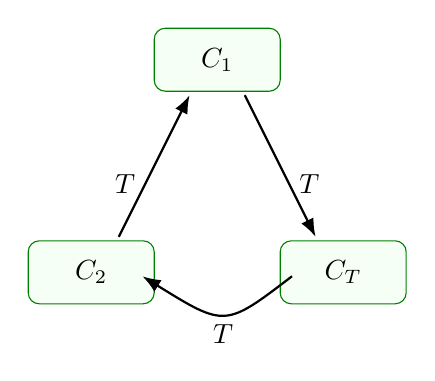
\begin{tikzpicture}[>=Latex, scale=1.0]
\coordinate (A) at (0,1.7);
\coordinate (B) at (-1.6,-1.0);
\coordinate (C) at (1.6,-1.0);
\node[draw=green!50!black, fill=green!4, rounded corners, minimum width=1.6cm, minimum height=0.8cm] at (A) {$C_1$};
\node[draw=green!50!black, fill=green!4, rounded corners, minimum width=1.6cm, minimum height=0.8cm] at (B) {$C_2$};
\node[draw=green!50!black, fill=green!4, rounded corners, minimum width=1.6cm, minimum height=0.8cm] at (C) {$C_T$};
\draw[->, thick] ($(A)+(0.35,-0.45)$) .. controls (0.95,0.05) .. ($(C)+(-0.35,0.45)$) node[midway, right] {$T$};
\draw[->, thick] ($(C)+(-0.65,-0.05)$) .. controls (0.1,-1.7) .. ($(B)+(0.65,-0.05)$) node[midway, below] {$T$};
\draw[->, thick] ($(B)+(0.35,0.45)$) .. controls (-0.95,0.05) .. ($(A)+(-0.35,-0.45)$) node[midway, left] {$T$};
\end{tikzpicture}
\caption{Family monodromy triangle. This is treated as a Bridge whose full theorem is still pending.}
\label{fig:family-triangle}
\end{figure}

A stronger geometric realization would replace this three-dimensional marker space by a flat $\mathbb Z_3$ local system, or better an $SU(3)$ family local system, on the seam complement.

\begin{proposition}[Family count from patch deficit]
The fundamental section of the seam complement has $F_{\mathrm{patch}}=4$ local corner patches. Each patch carries a spin-lifted deficit factor $1-\frac14=\frac34$. The resulting family multiplicity is
\begin{equation}
\label{eq:family-patch-deficit}
N_{\mathrm{fam}}=F_{\mathrm{patch}}\!\left(1-\frac14\right)=4\cdot\frac34=3.
\end{equation}
\end{proposition}

\begin{proof}[Proof sketch]
The fundamental domain of the seam complement is bounded by four corner regions where the local geometry meets the boundary of the fundamental section. Each corner carries a cone-angle deficit of $2\pi/4=\pi/2$. The spin lift doubles the covering, so each corner contributes a fractional chiral sector of weight $1-\frac{1}{4}=\frac{3}{4}$ rather than a full unit. The total number of independent chiral sectors is therefore $4\cdot\frac{3}{4}=3$. This is the same patch-and-deficit mechanism that produces $\deltatop$ in the topological surcharge; here it counts families rather than defect weight.
\end{proof}

This is the same multiplicity as the cycle count of the monodromy triangle; the two routes are therefore mutually overdetermined. The global route gives $N_{\mathrm{fam}}$ as a monodromy count, the local route gives $N_{\mathrm{fam}}$ as a patch-deficit count. If both close, the family number is locked from two independent directions. Once $N_{\mathrm{fam}}=3$ is accepted, the remaining family-side statement is immediate:
\[
\Oadm=N_{\mathrm{fam}}\dim S^+=3\times 16=48,
\]
and the topological surcharge becomes a corollary rather than a second postulate:
\[
\deltatop=\Oadm\,\cthree^4.
\]
The full theorem of monodromy---i.e.\ deriving $F$ as a local system from the seam cycle algebra---remains part of the bridge program, but the family count itself is now supported by both a global and a local argument.

\subsection{Occupancy and boundary-to-bulk transgression}

With the family bridge installed, the matter space becomes $S^+\otimes F$ and the occupancy $\Oadm=48$ is already fixed by the preceding proposition. Here \emph{occupancy} means the admissible chiral-state count after family lifting; it is not used as a primitive datum. The bridge point is not that family lifting creates a new numerical surcharge. Rather, the inherited hard kernel value
\[
\deltatop=\frac{3}{256\pi^4}
\]
admits on the canonical family branch the occupancy reinterpretation $\deltatop=\Oadm\,\cthree^4$.
Likewise the hard second-order defect contribution is re-read as
\[
\delta_2=\frac54\,\deltatop^2=B\gamma\,\Oadm^2\cthree^8.
\]
This bridge reinterpretation is the boundary-to-bulk step that later feeds both the electromagnetic and geometric benchmark channels. The coefficient $5/4$ is therefore not an extra numerical motif; it is the minimal-carrier compression factor $B\gamma$ rewritten in defect language. At the same time, the equality $\deltatop=\Oadm\cthree^4$ should be read exactly as a bridge reinterpretation, not yet as a proved transgression theorem in the ordinary field-theory sense.

\subsection{From bridge to geometric completion}

\begin{principle}[Completion split]
Once the carrier packet and family bridge are fixed, the focused main-text completion problem splits into a geometric program $\Ageom$ and a transport program $\Atrans$. Record algebra is retained only as a conditional appendix layer in \Cref{app:record}.
\end{principle}

The two main-text programs are packaged as
\[
\Ageom
:=
\langle E_3\oplus E_2,\ \chi,\ \mathcal B_{\mathrm{rel}},\ g,\ \omega_{\mathrm{spin}}\rangle,
\qquad
\Atrans
:=
\langle U_6,\ T,\ D_y,\ \mathcal Y_y^{(\varepsilon)},\ \mathcal C_{\Seam}\rangle.
\]
This split keeps the carrier theorem, the geometric closure problem, and the record-level extensions from being flattened into one undifferentiated claim.

\subsection{Relative APS and superconnection setup}

The geometric completion is formulated on a graded bundle
\[
\mathcal E_{\mathrm{rel}}=\mathcal E_{\mathrm{rel}}^+\oplus\mathcal E_{\mathrm{rel}}^-,
\]
with a declared reference pair $(D,D_{\mathrm{ref}})$ and APS-type boundary conditions on the seam $\Seam$; see Appendix~\ref{app:aps}. The geometric package is
\[
\mathbb A_{\Seam}:=D_{\mathrm{rel}}\oplus\mathcal B_{\mathrm{rel}}\oplus\nabla_\chi.
\]
This is a \emph{construction}, not yet a theorem. Its value is to keep grading, reference subtraction, seam data, and the $\chi$ channel in one object from the start rather than mixing them only at the level of later heuristics.

\subsection{Bosonic relative index and Higgs selection}

\begin{conjecture}[Bosonic relative index closure]
The bosonic relative index satisfies
\[
\Ind_{\mathrm{rel}}^{\mathsf{Adm}}(\mathcal B_{E_2}^+)=1,
\qquad
\Ind_{\mathrm{rel}}^{\mathsf{Adm}}(\mathcal B_{E_3}^+)=0.
\]
Consequently the unique light seam-even bosonic zero mode lies in
\[
\Phi\in\Gamma(E_2)\cong (1,2)_{1/2},
\qquad
\inv\Phi=+\Phi.
\]
\end{conjecture}

This is the sharp form of the Higgs claim used here. The issue is not whether a Higgs doublet can be written down, but whether the relative bosonic index can be shown to select it uniquely.
If that selection theorem closes, the renormalizable carrier-compatible Yukawa couplings are the standard ones,
\[
Q\,u^c\,\Phi,
\qquad
Q\,d^c\,\Phi^\dagger,
\qquad
L\,e^c\,\Phi^\dagger,
\qquad
L\,\nu^c\,\Phi,
\]
so the Higgs statement becomes a genuine structural bridge rather than a notation choice.

\subsection{Heat-kernel coefficient map and \texorpdfstring{$\chi$}{chi} bifurcation}

The local target action is written as
\begin{equation}
\label{eq:chi-effective-action}
\begin{aligned}
\Gammaeff
=
\int d^4x\sqrt{-g}\,
\Big[
c_R\chi^2R
+Z_\chi(\partial\chi)^2
-\mu_\Phi^2(\chi)\,\Phi^\dagger\Phi
+\lambda_\Phi(\Phi^\dagger\Phi)^2
+\frac{1}{6M^2}R^2
+\cdots
\Big].
\end{aligned}
\end{equation}
The coefficient bookkeeping expected from the relative spectral expansion is summarized in \Cref{tab:heat-kernel-map}.

\begin{table}[t]
\centering
\small
\begin{tabularx}{\linewidth}{@{}>{\raggedright\arraybackslash}p{0.15\linewidth}>{\raggedright\arraybackslash}p{0.22\linewidth}>{\raggedright\arraybackslash}p{0.22\linewidth}>{\raggedright\arraybackslash}p{0.14\linewidth}>{\raggedright\arraybackslash}p{0.14\linewidth}@{}}
\toprule
Coefficient & Operator sector & Generated term & $\chi$ scaling & Status \\
\midrule
$a_0$ & relative bulk trace & vacuum-energy bookkeeping & $\chi^4$ & Hard \\
$a_2$ & even bulk term & $\chi^2R$, mass-type terms & $\chi^2$ & Completion \\
$a_4$ & local curvature and scalar sector & $(\partial\chi)^2$, $\Phi^\dagger\Phi$, $(\Phi^\dagger\Phi)^2$, $R^2$ & $\chi^0$ & Completion \\
boundary/defect term & seam correction and parity data & local defect counterterms, seam-even selection & $\Delta_{\Seam}$ & Bridge \\
$\eta$ term & APS spectral asymmetry & sign and spectral-flow control & scale free & Bridge \\
\bottomrule
\end{tabularx}
\caption{Heat-kernel map for the geometric completion program.}
\label{tab:heat-kernel-map}
\end{table}

The resulting geometric logic is displayed in \Cref{fig:chi-bifurcation}. The same scale channel is asked to speak both to the induced Einstein term and to the scalar vacuum response. This is why the $\chi$ sector is the principal unresolved geometric closure problem.

\begin{figure}[t]
\centering
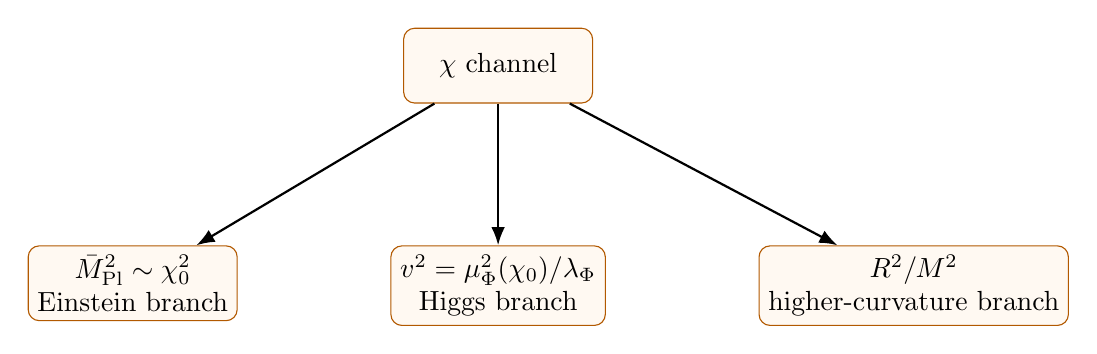
\begin{tikzpicture}[
    >=Latex,
    node distance=1.8cm and 2.1cm,
    box/.style={draw=orange!70!black, rounded corners, fill=orange!5, align=center, minimum width=2.4cm, minimum height=0.95cm}
]
\node[box] (chi) {$\chi$ channel};
\node[box, below left=of chi] (einstein) {$\Mpl^2\sim \chi_0^2$\\Einstein branch};
\node[box, below=of chi] (higgs) {$v^2=\mu_\Phi^2(\chi_0)/\lambda_\Phi$\\Higgs branch};
\node[box, below right=of chi] (r2) {$R^2/M^2$\\higher-curvature branch};
\draw[->, thick] (chi) -- (einstein);
\draw[->, thick] (chi) -- (higgs);
\draw[->, thick] (chi) -- (r2);
\end{tikzpicture}
\caption{Bifurcation of the $\chi$ channel. The three arrows are treated as one coupled geometric completion problem rather than as independent numerical inputs.}
\label{fig:chi-bifurcation}
\end{figure}

\begin{conjecture}[Induced Einstein and vacuum channel]
On the canonical branch the relative heat-kernel closure yields
\begin{equation}
\label{eq:induced-einstein}
\Mpl^2=\frac{\chi_0^2}{2\pi^2},
\qquad
v^2=\frac{\mu_\Phi^2(\chi_0)}{\lambda_\Phi}.
\end{equation}
\end{conjecture}

\begin{remark}[Newton form is not an independent output]
Using the standard reduced-Planck definition $\Mpl^{-2}=8\pi G_N$, the first relation in \Cref{eq:induced-einstein} is equivalently
\[
G_N\chi_0^2=\frac{\pi}{4}.
\]
This Newton-form equation is therefore a rewriting of the Einstein-branch closure, not a second independent prediction.
\end{remark}

\begin{conjecture}[Carrier-dressed electroweak vacuum]
If the $\chi$-channel Higgs mass parameter inherits the carrier rank and transport seed, the sharpest conditional target formula is
\begin{equation}
\label{eq:carrier-dressed-v}
v
=
\Mpl\,\gcar\,\beta_{\mathrm{rad}}^2\,
\exp\!\left(-\frac{\alpha^{-1}(0)}{5}\right)
\exp\!\left(-\frac{\delta_{\mathrm{ph}}}{5}\right),
\end{equation}
where $\gcar=5$ is the carrier rank and $\delta_{\mathrm{ph}}=\frac35+\frac{\phiz}{6}$ is the transport bridge offset defined in \Cref{eq:transport-bridge-offset}. This makes the electroweak vacuum a carrier-rank-weighted, $\alpha$-suppressed, transport-corrected fraction of the Planck scale, and turns the v2.8 constant-factory observation into a theorem candidate once the $a_2$/$a_4$ heat-kernel coefficients are computed in a declared scheme.
\end{conjecture}

\begin{remark}[Sector-dressed \texorpdfstring{$\chi$}{chi} channels]
The quantity $\chi_0$ entering the induced Einstein channel is not identified with the transport-sector confinement scale. In the hadronic sector we write $\chi_{\QCD}$ and regard it as a locally dressed channel obtained from the same underlying $\chi$ response after sector-dependent renormalization and confinement-scale matching:
\[
\chi \longrightarrow \chi_0 \quad \text{(gravitational background)},
\qquad
\chi \longrightarrow \chi_{\QCD} \quad \text{(transport-dressed local channel)}.
\]
This is the minimal statement needed to avoid the otherwise immediate scale clash between the Planck bridge and the QCD string tension.
\end{remark}

The E$_8$ scale ladder is not used as a primitive input in the main text. Only its short downstream grammar is retained in the dedicated main-text section, while the fuller arithmetic continuations are deferred to Appendix~\ref{app:constants}.

\section{Completion program B: Yukawas, masses, flavor, confinement, and strong CP}

The second completion block is the transport compiler. Its role is to turn the carrier packet and the family/occupancy bridge into actual masses, mixings, hadronic admissibility, and strong-CP control. The logic is again staged: first the discrete phase operator and the transport kernel, then path-length masses and mixing data, then confinement and strong CP as transport-side admissibility statements.

\subsection{Discrete phase operator and transport grammar}

Let
\[
\omega=e^{2\pi i/3},
\qquad
U_6=\mathrm{diag}(1,\omega,\omega^2,-1,-\omega,-\omega^2).
\]
This makes the phase grammar concrete rather than rhetorical. The six admissible phases are shown in \Cref{fig:z6-circle}, and CP acts by inversion $\delta\mapsto-\delta$ on this circle.

\begin{remark}[Hexagonal spectral geometry]
The operator $U_6$ is a unitary circulant with eigenphases $e^{in\pi/3}$ for $n=0,\dots,5$. The transport kernel $D_y=y\,\mathbf 1-\delta_{\mathrm{ph}}U_6$ is therefore a spectral problem on the discrete $C_6$ cycle. CKM and PMNS mixings, mass hierarchies, and the Möbius quotients of \Cref{eq:mobius-quotient} are then not loose analytic fits but spectral-theory statements on a regular hexagon. The near-pole hierarchy at $y\approx\delta_{\mathrm{ph}}$ becomes the resonance of a hexagonal resolvent rather than tuned parameter choice.
\end{remark}

\begin{figure}[t]
\centering
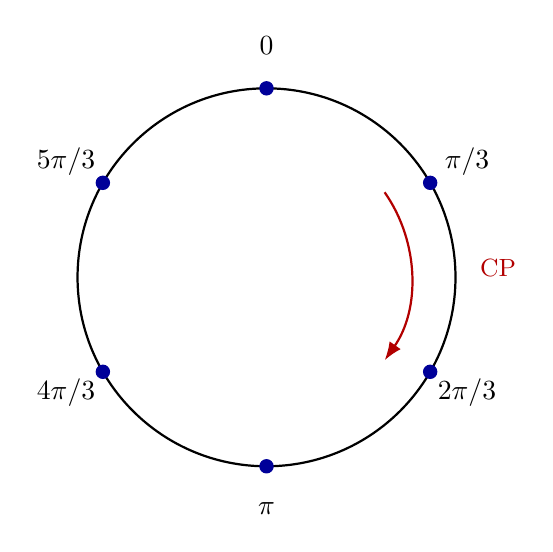
\begin{tikzpicture}[scale=1.2,>=Latex]
\draw[thick] (0,0) circle (2.0);
\foreach \ang/\lab in {90/{0},30/{\pi/3},-30/{2\pi/3},-90/{\pi},-150/{4\pi/3},150/{5\pi/3}} {
    \filldraw[blue!60!black] ({2*cos(\ang)},{2*sin(\ang)}) circle (2pt);
    \node at ({2.45*cos(\ang)},{2.45*sin(\ang)}) {$\lab$};
}
\draw[->,red!70!black,thick] (1.25,0.9) arc[start angle=35,end angle=-35,radius=1.55];
\node[red!70!black] at (2.45,0.1) {\small CP};
\end{tikzpicture}
\caption{$\mathbb Z_6$ phase circle with CP inversion.}
\label{fig:z6-circle}
\end{figure}

\subsection{Regularized Yukawa kernels and path-length masses}

Here
\begin{equation}
\label{eq:transport-bridge-offset}
\delta_{\mathrm{ph}}:=\frac35+\frac{\phiz}{6}
\end{equation}
is treated as a transport bridge parameter inherited from the cross-ratio and boundary-monodromy program, rather than as a proved hard-kernel identity. The full derivation is therefore deferred to the supplementary layer, while the regularized transport operator used here is
\begin{equation}
\label{eq:yukawa-kernel}
\begin{aligned}
D_y&=y\,\mathbf 1-\delta_{\mathrm{ph}}U_6,\\
\mathcal Y_y^{(\varepsilon)}&=(D_y^\dagger D_y+\varepsilon^2)^{-1},
\end{aligned}
\end{equation}
and the singular limit $\varepsilon\to0$ is taken only in admissible sectors.

Because $U_6$ has eigenphases $e^{in\pi/3}$, the regularized transport spectrum is
\begin{equation}
\label{eq:transport-spectrum}
\lambda_{y,n}^{-1}
=
y^2+\delta_{\mathrm{ph}}^2-2y\delta_{\mathrm{ph}}\cos\!\left(\frac{n\pi}{3}\right)+\varepsilon^2,
\qquad
n=0,\dots,5,
\end{equation}
for the eigenvalues $\lambda_{y,n}$ of $\mathcal Y_y^{(\varepsilon)}$. In particular,
\begin{equation}
\label{eq:mobius-quotient}
\frac{\lambda_{y,0}}{\lambda_{y,3}}
=
\left(\frac{y+\delta_{\mathrm{ph}}}{y-\delta_{\mathrm{ph}}}\right)^2.
\end{equation}
\begin{remark}[Near-pole hierarchy mechanism]
On the retained branch
\[
\delta_{\mathrm{ph}}=\frac35+\frac{\phiz}{6}\approx \num{0.60886}.
\]
Hence the Möbius quotient contains a built-in near-pole whenever $y$ approaches $\delta_{\mathrm{ph}}$, making large hierarchy ratios structurally plausible. At present this is a hierarchy mechanism, not yet a theorem of explanatory control: until admissible path lengths $L_{f,j}$ and bounded residual factors $\Lambda_{f,j}$ are derived geometrically, the same near-pole can also masquerade as a tuning surface.
\end{remark}

Absolute masses are attached to admissible path lengths,
\begin{equation}
\label{eq:path-length-yukawa}
y_{f,j}^{\mathrm{UV}}=\lambdaY^{L_{f,j}}\Lambda_{f,j},
\qquad
\lambdaY=\sqrt{\phiz(1-\phiz)}.
\end{equation}
After the electroweak bridge fixes $v$, the physical mass rows are emitted through
\begin{equation}
\label{eq:mass-bridge}
m_{f,j}=\frac{y_{f,j}v}{\sqrt2}.
\end{equation}
The role of the residual factors $\Lambda_{f,j}$ must be kept explicit. They are bounded $O(1)$ transport prefactors, not unrestricted fit knobs.

\begin{remark}[Flavor cusps as carrier cusps]
The admissible cusp values $y\in\{1,\frac13,\frac23\}$ are not arbitrary rational points; they are the absolute values of the singular hypercharges $|Y(e^c)|=1$, $|Y(d^c)|=\frac13$, $|Y(u^c)|=\frac23$. The transport grammar therefore lives on the same rational grid as the carrier packet itself.
\end{remark}

On the minimal admissible branch the word-length candidates are
\begin{equation}
\label{eq:minimal-word-lengths}
\begin{gathered}
L_t=0,\quad
L_b=L_\tau=3,\quad
L_c=4,\quad
L_s=L_\mu=5,\\
L_d=7,\quad
L_u=L_e=8.
\end{gathered}
\end{equation}
These are not free parameters; they are the minimal admissible word lengths on the $C_6$ graph that reproduce the observed mass hierarchy through $\lambdaY^{L_{f,j}}$. The assignment is unique up to residual-factor control: once the hierarchy ordering is fixed, the nearest-integer graph distance is determined by $\lambdaY\approx\num{0.2244}$.

The transport-side status is summarized in \Cref{tab:transport-dictionary}.

\begin{table}[t]
\centering
\scriptsize
\resizebox{\linewidth}{!}{%
\begin{tabular}{@{}lllll@{}}
\toprule
Sector & Admissible length data & Residual prefactor & Role & Status \\
\midrule
charged leptons & $L_{e}=8,\;L_\mu=5,\;L_\tau=3$ & $\Lambda_e,\Lambda_\mu,\Lambda_\tau$ & ladder and hierarchy & bounded; operator closure open \\
up quarks & $L_u=8,\;L_c=4,\;L_t=0$ & $\Lambda_u,\Lambda_c,\Lambda_t$ & up-type ratio ladder & bounded; phase closure open \\
down quarks & $L_d=7,\;L_s=5,\;L_b=3$ & $\Lambda_d,\Lambda_s,\Lambda_b$ & down-type ratio ladder & bounded; phase closure open \\
quark mixing & $L_{ij}^{q}$ & $\Lambda_{ij}^{q}$ & CKM transport entries & bounded; phase closure open \\
neutrino mixing & $L_{ij}^{\nu}$ & $\Lambda_{ij}^{\nu}$ & PMNS transport entries & bounded; bridge partial \\
hadron basis & center-neutral word lengths & block coefficients & meson and baryon transport basis & open bound-state layer \\
strong CP & determinant spectrum of $\mathcal Y_f$ & none if positivity closes & phase suppression & positivity hardening pending \\
\bottomrule
\end{tabular}}
\caption{Transport algebra dictionary with minimal admissible word-length candidates.}
\label{tab:transport-dictionary}
\end{table}

\subsection{CKM and PMNS sharpening}

The leading CKM magnitudes on the transport branch are
\begin{equation}
\label{eq:ckm-magnitudes}
s_{12}=\lambda_C,
\qquad
s_{23}=\frac{\phiz}{1+\lambda_C},
\qquad
s_{13}=\frac{\lambda_C^3}{3}.
\end{equation}
The CKM phase receives a tri-familial dressing beyond the raw topological $\pi/3$:
\begin{equation}
\label{eq:ckm-phase}
\delta_{\mathrm{CKM}}=\frac{\pi}{3}+3\lambda_C^2\approx\num{1.198}\;\mathrm{rad},
\end{equation}
so $\pi/3$ remains the base monodromy phase and $3\lambda_C^2$ is the leading family-transport correction.

For the neutrino sector the minimal seesaw closure on the transport branch is
\begin{equation}
\label{eq:neutrino-masses}
m_3=e^{2\lambda_C^2}\frac{v^2}{M_R},
\qquad
m_2=\pi\phiz\,m_3,
\qquad
m_1=0,
\end{equation}
with $M_R\approx\num{1.31e15}\;\mathrm{GeV}$ fixed by the seesaw E$_8$ block at $(n,r,I_1)=(5,5,\frac{1}{12})$. Numerically this gives
\[
m_3\approx\num{0.0508}\;\mathrm{eV},
\qquad
m_2\approx\num{0.0085}\;\mathrm{eV},
\]
consistent with normal ordering.

\subsection{Confinement as admissible word selection}

\begin{proposition}[Admissible color words]
For each carrier word $w$, let $z(w)\in\{1,\omega,\omega^2\}$ be its color-center charge and let $\varepsilon(w)\in\{\pm1\}$ be its seam parity. Physical hadronic words satisfy
\[
z(w)=1,
\qquad
\varepsilon(w)=+1.
\]
\end{proposition}

The confinement claim is thus stated as an admissibility rule, not as a late dynamical slogan. A schematic version is shown in \Cref{fig:admissible-words}.

\begin{figure}[t]
\centering
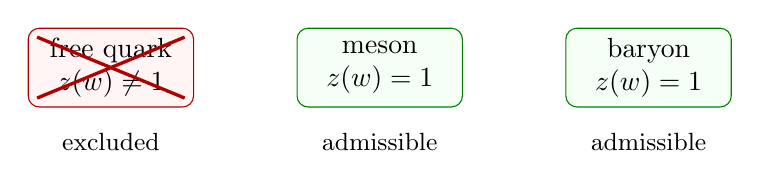
\begin{tikzpicture}[>=Latex, node distance=1.1cm and 1.3cm]
\node[draw=red!70!black, fill=red!4, rounded corners, minimum width=2.1cm, minimum height=1.0cm, align=center] (q) {free quark\\$z(w)\neq 1$};
\node[draw=green!50!black, fill=green!4, rounded corners, minimum width=2.1cm, minimum height=1.0cm, align=center, right=of q] (m) {meson\\$z(w)=1$};
\node[draw=green!50!black, fill=green!4, rounded corners, minimum width=2.1cm, minimum height=1.0cm, align=center, right=of m] (b) {baryon\\$z(w)=1$};
\draw[red!70!black, very thick] ($(q.north west)+(0.12,-0.12)$) -- ($(q.south east)+(-0.12,0.12)$);
\draw[red!70!black, very thick] ($(q.south west)+(0.12,0.12)$) -- ($(q.north east)+(-0.12,-0.12)$);
\node[below=0.2cm of q] {\small excluded};
\node[below=0.2cm of m] {\small admissible};
\node[below=0.2cm of b] {\small admissible};
\end{tikzpicture}
\caption{Confinement as admissible word selection.}
\label{fig:admissible-words}
\end{figure}

The transport-sector string tension is written as
\[
\sigma=\cthree^2\chi_{\QCD}^2,
\]
so the relative Wilson loop obeys
\[
\langle W(C)\rangle_{\mathrm{rel}}\sim e^{-\sigma A(C)}.
\]
The sector-dependent scale $\chi_{\QCD}$ is the minimal notation needed to avoid confusing the hadronic transport channel with the gravitational $\chi_0$ background; the two channels are linked by the common underlying $\chi$ response but not by a naive equality of scales.

\subsection{Strong CP closure as conditional steps}

Define
\begin{equation}
\label{eq:strong-cp}
\bar\theta=\theta_{\mathrm{sheet}}+\arg\det M_u+\arg\det M_d.
\end{equation}
The intended closure is decomposed into five conditional steps.

\begin{conditionalstep}[Sheet-odd cancellation]
The bare $G\widetilde G$ contribution is odd under the sheet exchange and cancels in the relative action, so $\theta_{\mathrm{sheet}}=0$ in the admissible relative sector.
\end{conditionalstep}

\begin{conditionalstep}[Positive radial kernel]
The regularized transport kernel induces a positive radial operator $H_f>0$ on the admissible sector, so the transport-side radial mass data carry no intrinsic determinant phase.
\end{conditionalstep}

\begin{conditionalstep}[Holonomy factorization]
The physical mass map admits a polar decomposition
\[
M_f=U_{f,L}H_fU_{f,R}^\dagger,
\qquad
U_{f,L},U_{f,R}\in SU(3)_F,
\]
where the unitary factors are family-holonomy transport matrices.
\end{conditionalstep}

\begin{conditionalstep}[Vanishing determinant phase with weak CP preserved]
If the physical mass map is defined by that positive radial branch and special-unitary holonomy data, then
\[
\arg\det M_f=0.
\]
At the same time
\[
V_{\mathrm{CKM}}=U_{u,L}^\dagger U_{d,L}
\]
may still carry a nontrivial Jarlskog invariant.
\end{conditionalstep}

\begin{conditionalstep}[RG preservation]
The vanishing of $\bar\theta$ is preserved under the declared RG and matching map as long as no phase-violating counterterm is inserted by hand.
\end{conditionalstep}

\begin{conjecture}[Conditional strong-CP closure]
Under the five conditional steps above,
\[
\bar\theta=0.
\]
\end{conjecture}

The positive-branch clause is essential here: the closure statement is about the physical mass map once the admissible transport branch has been fixed, not about an arbitrary unitary dressing of the same singular values. The point of the polar decomposition is precisely to separate strong and weak CP cleanly: the positive radial part fixes $\arg\det M_f=0$, while weak CP may survive through the relative family holonomies encoded in $V_{\mathrm{CKM}}$.

\begin{remark}[Admissibility as a unified three-sector motif]
The admissibility predicate $\mathsf{Adm}$ acts as a single structural principle with three sector projections:
\begin{itemize}[leftmargin=1.5em, topsep=3pt, itemsep=2pt]
    \item \textbf{Electroweak:} seam-even selection picks the unique light Higgs doublet ($\inv\Phi=+\Phi$).
    \item \textbf{QCD:} center neutrality selects confined hadronic words ($z(w)=1$, $\varepsilon(w)=+1$).
    \item \textbf{Strong CP:} sheet-odd cancellation kills $\theta_{\mathrm{sheet}}$ in the relative action.
\end{itemize}
These are not three independent rules bolted onto different sectors. They are three projections of the same admissible-versus-inadmissible boundary: seam parity, center charge, and sheet exchange are all encoded in the double-cover and involution data of the primitive core. This unification is the conceptual backbone of the transport program.
\end{remark}

\section{Particle and mass compiler}

This section is the phenomenological heart of the manuscript. It is not meant to flatten all rows into one uniform notion of prediction. Instead it makes the compiler interface explicit: a declared RG map, a kernel-output map, and a mass ledger that separates genuinely derived quantities from solver-level candidates and anchor-dependent comparison rows.
Accordingly this section is best read through three ledgers:
\begin{itemize}[leftmargin=1.5em, topsep=3pt, itemsep=2pt]
    \item a \emph{primary benchmark ledger} for the narrow main-text comparison surface in \Cref{tab:benchmark},
    \item \emph{mass-closure ledgers} for fermion, electroweak, and hadronic rows in \Cref{tab:sm-mass-ledger-ew,tab:sm-mass-ledger-quarks},
    \item and a \emph{supplementary / anchor-dependent ledger} in the appendix for rows that remain comparison-heavy or exploratory.
\end{itemize}

\subsection{RG map for compiler outputs}

The symbol $\mathcal R_{\SM}$ denotes the declared comparison map from TFPT outputs to scheme-specified observables. Here it is the bookkeeping package
\[
\mathcal R_{\SM}
=
\bigl(
\mu_{\mathrm{match}},\ \{\mu_{\mathrm{thr}}\},\ \text{running convention},\ \text{scheme conversion},\ \text{observable map}
\bigr),
\]
and we write
\[
\bar\alpha^{(5)}(M_Z):=\alpha_{\mathrm{em}}^{\overline{\mathrm{MS}},\,n_f=5}(M_Z).
\]
with the following restricted interpretation in the main text:
\begin{itemize}[leftmargin=1.5em, topsep=3pt, itemsep=2pt]
    \item $\alpha^{-1}(0)$ is compared in the Thomson-limit on-shell convention, with the CODATA 2022 / NIST value taken as the normative low-energy reference rather than the separate PDG electroweak extraction from $a_e$,
    \item $\bar\alpha^{(5)}(M_Z)^{-1}$ is compared after a declared threshold map into the $\overline{\mathrm{MS}}$ language at $\mu=M_Z$,
    \item neutrino-angle rows use the NuFIT normal-ordering reference snapshot based on data available through November 2025,
    \item the $\Omega_b$ row is reconstructed from the Planck 2018 base-$\Lambda$CDM pair $(\Omega_b h^2,H_0)$ via $\Omega_b=(\Omega_b h^2)/h^2$ with $h=H_0/100$,
    \item the $\beta$ row uses the Minami--Komatsu extraction from Planck 2018 polarization as the normative benchmark, while PR4 and PR4 map-space analyses are kept only as supplementary context,
    \item direct-search interface rows are not treated as precision residuals and are therefore kept out of the main benchmark table.
\end{itemize}
For later use we also set
\[
\beta_{\mathrm{rad}}:=\frac{\phiz}{4\pi}.
\]

\subsection{Central hard-kernel quantities}

The roles of $\cthree$ and $\phiz$ should not remain implicit. They are the central hard numeric quantities of the present main-text kernel. The downstream E$_8$ parameter $\kappa_{E8}$ is isolated in the next section rather than folded back into the kernel center.

\begin{table}[t]
\centering
\scriptsize
\setlength{\tabcolsep}{3pt}
\begin{tabularx}{\linewidth}{@{}>{\raggedright\arraybackslash}p{0.11\linewidth}>{\raggedright\arraybackslash}p{0.19\linewidth}>{\raggedright\arraybackslash}p{0.24\linewidth}X@{}}
\toprule
Quantity & Closed value & Role / status & Named outputs \\
\midrule
$\cthree$ & \makecell[l]{$1/(8\pi)$\\$=\num{0.03979}$} & Hard seam normalization & $\deltatop$, $C_{a\gamma\gamma}=-4\cthree$, $\sigma=\cthree^2\chi_{\QCD}^2$, $M/\bar M_{\mathrm{Pl}}=\sqrt{8\pi}\cthree^4$ \\
$\phiz$ & \makecell[l]{$\frac{1}{6\pi}+\frac{3}{256\pi^4}$\\$=\num{0.05317}$} & Hard corrected opening; bridge reinterpretation via $\deltatop=\Oadm\cthree^4$ & $\beta_{\mathrm{rad}}=\phiz/(4\pi)$, $\lambda_C=\sqrt{\phiz(1-\phiz)}$, $\sin^2\theta_{13}$, charged-lepton ladders \\
\bottomrule
\end{tabularx}
\caption{Central hard-kernel quantities and the main predictions they feed.}
\label{tab:kernel-output-map}
\end{table}

The most exposed closed formulas driven by these constants are those already displayed in \Cref{eq:kernel-benchmark-formulas}.

\subsection{Mass-closure ledgers}

For the mass surface itself the main text now uses only three row-level status words:
\emph{derived}, \emph{candidate}, and \emph{anchor-dependent}. The explicit candidate formulas, neutrino rows, and transport-ratio source data are moved to the appendix so that the main text shows a compact comparison-ready ledger rather than a mixed formula dump.

\begin{table}[p]
\centering
\scriptsize
\setlength{\tabcolsep}{3pt}
\begin{tabularx}{\linewidth}{@{}>{\raggedright\arraybackslash}p{0.10\linewidth}>{\raggedright\arraybackslash}p{0.27\linewidth}>{\raggedleft\arraybackslash}p{0.15\linewidth}>{\raggedleft\arraybackslash}p{0.15\linewidth}>{\raggedleft\arraybackslash}p{0.10\linewidth}>{\raggedright\arraybackslash}p{0.12\linewidth}@{}}
\toprule
Particle & TFPT source class & TFPT value & PDG value & Residual & Status \\
\midrule
$e$ & constant-factory candidate & \num{0.52096} MeV & \num{0.510999} MeV & $+1.95\%$ & candidate \\
$\mu$ & constant-factory candidate & \num{107.49} MeV & \num{105.658} MeV & $+1.73\%$ & candidate \\
$\tau$ & constant-factory candidate & \num{1.7688} GeV & \num{1.77686} GeV & $-0.45\%$ & candidate \\
\midrule
\multicolumn{6}{@{}l}{\textit{Calibration surface (anchor-dependent; zero residual = anchor consistency, not prediction):}} \\
$W^\pm$ & boundary EW input at $M_Z$ & \num{80.369} GeV & \num{80.369} GeV & $0.00\%$ & anchor \\
$Z$ & boundary EW input at $M_Z$ & \num{91.188} GeV & \num{91.188} GeV & $0.00\%$ & anchor \\
$H$ & boundary Higgs input & \num{125.25} GeV & \num{125.25} GeV & $0.00\%$ & anchor \\
\bottomrule
\end{tabularx}
\caption{Compact mass surface, electroweak and charged-lepton sector. Zero residual on anchor-dependent rows records consistency with the chosen anchor only.}
\label{tab:sm-mass-ledger-ew}
\end{table}

\begin{table}[p]
\centering
\scriptsize
\setlength{\tabcolsep}{3pt}
\begin{tabularx}{\linewidth}{@{}>{\raggedright\arraybackslash}p{0.10\linewidth}>{\raggedright\arraybackslash}p{0.27\linewidth}>{\raggedleft\arraybackslash}p{0.15\linewidth}>{\raggedleft\arraybackslash}p{0.15\linewidth}>{\raggedleft\arraybackslash}p{0.10\linewidth}>{\raggedright\arraybackslash}p{0.12\linewidth}@{}}
\toprule
Particle & TFPT source class & TFPT value & PDG value & Residual & Status \\
\midrule
$u$ & light-quark solver relative to strange anchor, $\overline{\mathrm{MS}}$ at $2$ GeV & \num{2.195} MeV & \num{2.16} MeV & $+1.62\%$ & derived \\
$d$ & light-quark solver relative to strange anchor, $\overline{\mathrm{MS}}$ at $2$ GeV & \num{4.67} MeV & \num{4.67} MeV & $+0.00\%$ & derived \\
$\pi^0$ & GMOR hadronic cross-check & \num{134.979} MeV & \num{134.977} MeV & $+0.00\%$ & derived \\
$p$ & hadron mass-ladder cross-check & \num{935.03} MeV & \num{938.272} MeV & $-0.35\%$ & derived \\
\midrule
\multicolumn{6}{@{}l}{\textit{Calibration surface (anchor-dependent):}} \\
$s$ & strange-quark anchor, $\overline{\mathrm{MS}}$ at $2$ GeV & \num{93.4} MeV & \num{93.4} MeV & $0.00\%$ & anchor \\
$c$ & up-type ratio ladder with threshold input & \num{1.27} GeV & \num{1.27} GeV & $0.00\%$ & anchor \\
$b$ & down-type ratio ladder with threshold input & \num{4.18} GeV & \num{4.18} GeV & $0.00\%$ & anchor \\
$t$ & up-type ratio ladder with threshold input & \num{172.57} GeV & \num{172.57} GeV & $0.00\%$ & anchor \\
\bottomrule
\end{tabularx}
\caption{Compact mass surface, quark and first-hadron sector. Zero residual on anchor-dependent rows records consistency with the chosen anchor only.}
\label{tab:sm-mass-ledger-quarks}
\end{table}

The compact ledgers are intentionally narrow: they show the comparison surface, not the internal algebra. Explicit candidate formulas for $e,\mu,\tau$, neutrino branch values, and the ladder / ratio source rows for the quark sector are collected in the appendix-level supplementary mass-source table \Cref{tab:mass-source-supplement}.

\section{\texorpdfstring{E$_8$}{E8} as downstream scale grammar}

E$_8$ is not part of the primitive carrier ontology and should not compete with the seam data, the carrier theorem, or the completion program for explanatory priority. In the present main-text form it plays one restricted role only: a downstream scale grammar attached to the already fixed carrier norm.
\[
\kappa_{E8}:=\frac{\gamma}{\ln(248/60)}=\frac{5/6}{\ln(248/60)}.
\]

\subsection{Block formula and reading discipline}

A physical E$_8$ representation is not the stage label $n$ alone, but the full block triple $(n,r,I_1)$. The compressed block formula is
\begin{equation}
\label{eq:e8-block-formula}
X(n,r,I_1)
=
\frac{\Mplunred}{8}\,\sin^2\theta_{13}\,
\left(\frac{60-2n}{60}\right)^{\!\kappa_{E8}}
e^{-(8-r)/64}\,
e^{-12\pi I_1},
\end{equation}
where $\Mplunred\approx\num{1.2209e19}\;\mathrm{GeV}$ is the \emph{unreduced} Planck mass (not $\Mpl=\Mplunred/\sqrt{8\pi}$), $n$ is the ladder stage with $D_n=60-2n$, $r$ is a mild block-multiplicity label ($1\le r\le 8$), and $I_1$ is the dominant block trace. The reading discipline is strict: $n$ orders the ladder, $I_1$ controls most of the exponential suppression via $e^{-12\pi I_1}$, and $r$ only refines the scale. In the relevant energy range the step ratio between successive stages is
\[
\frac{X_{n+1}}{X_n}=\left(\frac{58-2n}{60-2n}\right)^{\!\kappa_{E8}}\approx 0.96\text{--}0.97,
\]
so large hierarchies come almost entirely from $I_1$, not from $n$.

\subsection{Restricted stage atlas}

With the restrictive trace grammar $I_1\in\{\frac{1}{12},\frac{1}{6},\frac{1}{3},\frac{1}{2},\frac{5}{8},\frac{41}{48},1,\frac{17}{16}\}$ the ladder produces a set of robust stage identifications. The main-text table shows only the robust nodes; the full real-domain atlas up to $n=29$---including restricted-scan candidates and IR tail conjectures---is given in \Cref{tab:e8-full-atlas} in the appendix.

\begin{table}[t]
\centering
\scriptsize
\setlength{\tabcolsep}{3pt}
\begin{tabularx}{\linewidth}{@{}>{\centering\arraybackslash}p{0.04\linewidth}>{\centering\arraybackslash}p{0.04\linewidth}>{\raggedright\arraybackslash}p{0.07\linewidth}>{\raggedleft\arraybackslash}p{0.14\linewidth}>{\raggedleft\arraybackslash}p{0.14\linewidth}>{\raggedright\arraybackslash}p{0.10\linewidth}Y@{}}
\toprule
$n$ & $r$ & $I_1$ & $X$ (GeV) & Target & Residual & Identification \\
\midrule
$3$ & $8$ & $1/2$ & $\num{2.159e8}$ & $\num{2.160e8}$ & $0.06\%$ & $\mu_{\cthree}$ RG crossing \\
$5$ & $5$ & $1/12$ & $\num{1.307e15}$ & $\num{1.31e15}$ & $0.2\%$ & seesaw $M_R$ \\
$10$ & $1$ & $1/3$ & $\num{8.826e10}$ & direct search & --- & PQ scale $f_a$ \\
$12$ & $2$ & $41/48$ & $\num{246.35}$ & $\num{246.22}$ & $0.05\%$ & EW vacuum $v$ \\
$14$ & $4$ & $17/16$ & $\num{0.0921}$ & $\num{0.0927}$ & $0.6\%$ & pion band \\
$15$ & $4$ & $1$ & $\num{0.935}$ & $\num{0.938}$ & $0.3\%$ & hadron anchor \\
$21$ & $4$ & $1/6$ & $\num{3.051e13}$ & $\num{3.06e13}$ & $0.3\%$ & inflation $M$ \\
$21$ & $5$ & $41/48$ & $\num{171.8}$ & $\num{172.6}$ & $0.4\%$ & top quark \\
$24$ & $7$ & $5/8$ & $\num{7.895e5}$ & $\num{7.920e5}$ & $0.3\%$ & $\mu_{\phiz}$ RG crossing \\
$25$ & $5$ & $1$ & $\num{0.498}$ & $\num{0.498}$ & $0.0\%$ & kaon band \\
$25$ & $7$ & $41/48$ & $\num{125.5}$ & $\num{125.25}$ & $0.2\%$ & Higgs mass \\
$26$ & $2$ & $1$ & $\num{0.417}$ & $\num{0.42}$ & $0.7\%$ & $\sqrt{\sigma}$ confinement \\
\bottomrule
\end{tabularx}
\caption{Robust E$_8$ stage atlas (restrictive trace grammar only). Restricted-scan candidates and tail conjectures are in \Cref{tab:e8-full-atlas}.}
\label{tab:e8-stage-atlas}
\end{table}

\begin{remark}[Non-independence of stage-atlas entries]
The stage-atlas entries are not statistically independent confirmations. They are projections of a single block grammar $X(n,r,I_1)$ with three discrete parameters. The grammar organizes scale ratios once the carrier and transport seeds are fixed, but the number of ``hits'' is bounded by the number of $(n,r,I_1)$ triples that can be formed, not by the number of independent physical measurements. This is the scale-grammar analogue of the one-seed warning for the benchmark bridge rows.
\end{remark}

\subsection{Split-node structure}

Two stages carry a particularly revealing double structure.

\begin{proposition}[Inflation--top split node]
At $n=21$, the E$_8$ block formula admits two well-separated physical identifications:
\[
X(21,4,\tfrac16)\approx\num{3.051e13}\;\mathrm{GeV}\quad(\text{inflation scale}),
\qquad
X(21,5,\tfrac{41}{48})\approx\num{171.8}\;\mathrm{GeV}\quad(\text{top mass}).
\]
The same orbit depth carries the UV and IR endpoints of the electroweak hierarchy.
\end{proposition}

\begin{proposition}[Higgs--kaon split node]
At $n=25$, the block formula admits
\[
X(25,7,\tfrac{41}{48})\approx\num{125.5}\;\mathrm{GeV}\quad(\text{Higgs mass}),
\qquad
X(25,5,1)\approx\num{0.498}\;\mathrm{GeV}\quad(\text{kaon band}).
\]
Again a single orbit depth carries two widely separated physical sectors, distinguished entirely by the block trace $I_1$.
\end{proposition}

The split-node structure shows that $n$ is a radial orbit coordinate and $I_1$ is the sector projection. A physical representation of the E$_8$ ladder is therefore $(n,r,I_1)$, not $n$ alone.

\subsection{Permissiveness barrier and real-domain boundary}

\begin{remark}[Permissiveness barrier at $n=18{,}19$]
Under the restricted trace grammar, stages $n=18$ and $n=19$ have no unambiguous physical target. If $I_1$ is allowed to scan over all simple rationals, these stages can mimic almost any scale between $10^2$ and $10^{16}$~GeV. They mark the exact boundary where E$_8$ without a derived block-trace theorem becomes too permissive. The open key question of the E$_8$ layer is therefore not the ladder itself but the derivation of $I_1(B)$ from carrier and block structure. Until that derivation is available, stages $18$ and $19$ are the sharpest internal test points.
\end{remark}

\begin{remark}[Real-domain theorem]
The hard nilpotent chain gives $D_n=60-2n$ for $n=1,\dots,26$. Real-valued continuation is possible up to $n=29$ ($D_{29}=2>0$). At $n=30$, $D_n=0$ and the power $(D_n/60)^{\kappa_{E8}}$ hits a terminal wall. For $n\ge31$, $D_n<0$ and the irrational exponent $\kappa_{E8}$ produces complex values. The physically meaningful real-valued ladder therefore terminates at $n=29$.
\end{remark}

\begin{table}[t]
\centering
\small
\begin{tabularx}{\linewidth}{@{}>{\raggedright\arraybackslash}p{0.22\linewidth}>{\raggedright\arraybackslash}p{0.22\linewidth}Y@{}}
\toprule
Quantity & Value on the retained branch & Main-text role \\
\midrule
$\kappa_{E8}$ & \num{0.58723} & downstream ladder exponent fixed by $\gamma=5/6$ \\
$D_1$ & $60$ & optional ladder start index; arithmetically tied to the canonical branch \\
$f_a$ & $\num{8.86e10}\,\mathrm{GeV}$ & representative axion-side scale on the retained branch \\
$m_a$ & $\num{65.19}\,\mu\mathrm{eV}$ & representative downstream mass scale \\
$\nu_a$ & $\num{15.764}\,\mathrm{GHz}$ & representative frequency target \\
\bottomrule
\end{tabularx}
\caption{Short main-text E$_8$ parameter ledger. The role of E$_8$ here is organizational rather than ontological.}
\label{tab:e8-main-text}
\end{table}

\section{Primary benchmark map and prediction ledger}

The comparison values used in this section follow representative CODATA, PDG, NuFIT, Planck, and birefringence references \cite{codata2022,pdg2025,nufit2025,planck2018,minamiKomatsu2020,eskilt2023,sullivan2025}. The main-text table is intentionally restricted to six rows whose comparison language is already reasonably convention-complete. The compact mass surface is given separately in \Cref{tab:sm-mass-ledger-ew,tab:sm-mass-ledger-quarks}; more exploratory rows and the main unresolved comparison are moved to Appendix~\ref{app:benchmarks}.
Here \enquote{carrier closure} abbreviates the self-consistent electromagnetic closure expression with explicit $\phiz(\alpha)$ and second-order term $\delta_2=\frac54\deltatop^2$. The $\alpha^{-1}(0)$ row is therefore structurally different from the four bridge rows $(\beta,\Omega_b,\lambda_C,\sin^2\theta_{13})$, which are all projections of the same retained seed $\phiz$.

\begin{table}[t]
\centering
\scriptsize
\setlength{\tabcolsep}{2pt}
\resizebox{\linewidth}{!}{%
\begin{tabular}{@{}llrrrrll@{}}
\toprule
\makecell[l]{Obs.} & \makecell[l]{TFPT\\formula} & \makecell[r]{TFPT\\value} & \makecell[r]{Exp.\\value} & \makecell[r]{Unc.} & \makecell[r]{Residual} & \makecell[l]{Scale /\\scheme} & Status \\
\midrule
$\alpha^{-1}(0)$ & \makecell[l]{self-consistent carrier closure\\$\phiz(\alpha)$ and $\delta_2$} & \num{137.0359992} & \num{137.03599918} & \num{2.1e-8} & $+1.87\sigma$ & \makecell[l]{Thomson\\on-shell} & Hard \\
\makecell[l]{$\bar\alpha^{(5)}$\\$(M_Z)^{-1}$} & \makecell[l]{$\mathcal R_{\SM}$\\$[\alpha(0)]$} & \num{127.9405} & \num{127.93} & \num{0.008} & $+1.32\sigma$ & \makecell[l]{$\overline{\mathrm{MS}}$\\at $M_Z$} & Bridge \\
$\lambda_C$ & $\sqrt{\phiz(1-\phiz)}$ & \num{0.22438} & \num{0.22431} & \num{8.5e-4} & $+0.08\sigma$ & \makecell[l]{CKM\\proxy} & Bridge \\
$\sin^2\theta_{13}$ & \makecell[l]{$\phiz$\\$e^{-5/6}$} & \num{0.02311} & \num{0.02224} & \num{5.7e-4} & $+1.524\sigma$ & \makecell[l]{NuFIT\\NO} & Bridge \\
$\Omega_b$ & \makecell[l]{$(4\pi-1)$\\$\beta_{\mathrm{rad}}$} & \num{0.04894} & \num{0.04930} & \num{8.57e-4} & $-0.421\sigma$ & \makecell[l]{Planck 2018\\from $\Omega_b h^2$} & Bridge \\
$\beta$ & \makecell[l]{$\beta_{\mathrm{rad}}$\\in degrees} & \num{0.242} & \num{0.35} & \num{0.14} & $-0.77\sigma$ & \makecell[l]{Planck 2018\\Minami--Komatsu} & Bridge \\
\bottomrule
\end{tabular}}
\caption{Primary benchmark table for the main-text claims. Supplementary rows and out-of-sample checks are collected in Appendix~\ref{app:benchmarks}.}
\label{tab:benchmark}
\end{table}

\begin{remark}[One seed, four projections]
The bridge rows are not statistically independent hits. With
\[
\beta_{\mathrm{rad}}=\frac{\phiz}{4\pi},
\qquad
\Omega_b=(4\pi-1)\beta_{\mathrm{rad}},
\qquad
\lambda_C=\sqrt{\phiz(1-\phiz)},
\qquad
\sin^2\theta_{13}=\phiz e^{-\gamma},
\]
the four-row map is a one-variable seed map
\[
\mathcal S(\phiz):=\bigl(\beta_{\mathrm{rad}},\Omega_b,\lambda_C,\sin^2\theta_{13}\bigr),
\]
with Jacobian
\[
\frac{d\mathcal S}{d\phiz}
=
\left(
\frac{1}{4\pi},
\,
1-\frac{1}{4\pi},
\,
\frac{1-2\phiz}{2\sqrt{\phiz(1-\phiz)}},
\,
e^{-\gamma}
\right).
\]
Thus $\beta$, $\Omega_b$, $\lambda_C$, and $\sin^2\theta_{13}$ are one seed and four shadows, not four detached benchmark events. They remain in the table because their comparison conventions and uncertainty models differ, not because the underlying algebraic source is independent.
\end{remark}

\subsection{Compact prediction ledger}

The main benchmark table shows only a narrow comparison surface. To keep the compiler structure visible, \Cref{tab:prediction-ledger} summarizes which output packages belong to which layer of the paper.

\begin{table}[t]
\centering
\small
\begin{tabularx}{\linewidth}{@{}>{\raggedright\arraybackslash}p{0.18\linewidth}>{\raggedright\arraybackslash}p{0.12\linewidth}YY@{}}
\toprule
Domain & Status & Output package & Source layer \\
\midrule
Carrier packet & Hard & $E_3\oplus E_2$, $G_{\SM}^{\mathrm{glob}}$, $S^+$, $\gamma$, $\bone$ & minimal carrier theorem and half-spinor decomposition \\
Kernel numerics & Hard & $\cthree$, $\phiz$, $\alpha$, $C_{a\gamma\gamma}$, $\beta$, $\lambda_C$ & carrier-form closure equation and seam constants \\
Family / occupancy layer & Bridge & $F$, $\Oadm=48$, $\deltatop$ & monodromy and occupancy bridge \\
Geometric compiler & Completion & $\Phi$, $\Mpl$, $v$, $R^2$ channel & bosonic index plus relative heat-kernel closure \\
Transport compiler & Completion & $\mathcal Y_f$, $m_f$, CKM, PMNS & phase-distance kernel and path-length mass closure \\
QCD closure & Completion & confinement, hadronic admissibility, $\bar\theta=0$ & center neutrality plus positive-kernel hardening \\
Downstream ladder & Conditional & E$_8$ scale ratios and inflation-side imports & optional appendix-level scale grammar \\
Observer layer & Conditional & record algebra, horizons, prediction semantics & appendix-level extension \\
\bottomrule
\end{tabularx}
\caption{Compact prediction ledger for the carrier-first compiler presentation.}
\label{tab:prediction-ledger}
\end{table}

\subsection{Residual map and principal unresolved comparisons}

The residuals for the restricted six-row table are shown in \Cref{fig:residual-plot}. The carrier-linked electromagnetic, birefringence, and baryon-density channels all remain within the displayed few-sigma window. The CKM phase is not plotted here because it is better treated, at present, as the main unresolved transport-side comparison and is therefore moved to Appendix~\ref{app:benchmarks}.

\begin{figure}[t]
\centering
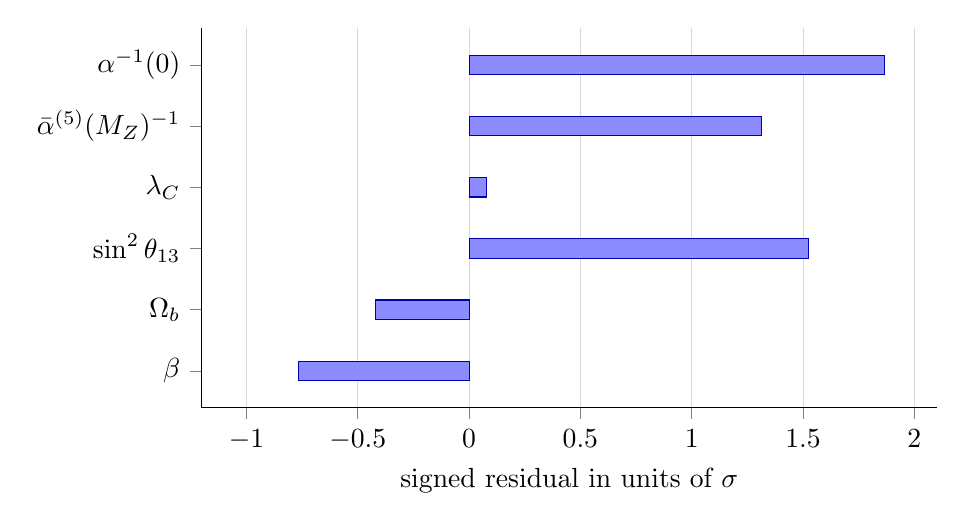
\begin{tikzpicture}
\begin{axis}[
    width=0.9\linewidth,
    height=6.4cm,
    xbar,
    bar width=7pt,
    xmin=-1.2,
    xmax=2.1,
    xlabel={signed residual in units of $\sigma$},
    symbolic y coords={beta,omegab,theta13,lambdac,alphaMZ,alpha0},
    ytick=data,
    yticklabels={$\beta$,$\Omega_b$,$\sin^2\theta_{13}$,$\lambda_C$,$\bar\alpha^{(5)}(M_Z)^{-1}$,$\alpha^{-1}(0)$},
    enlarge y limits=0.12,
    axis x line*=bottom,
    axis y line*=left,
    tick align=outside,
    major grid style={draw=gray!30},
    xmajorgrids=true
]
\addplot[fill=blue!45, draw=blue!70!black] coordinates {
    (-0.768,beta)
    (-0.421,omegab)
    (1.524,theta13)
    (0.078,lambdac)
    (1.315,alphaMZ)
    (1.865,alpha0)
};
\end{axis}
\end{tikzpicture}
\caption{Residual plot for the main benchmark rows with declared uncertainties.}
\label{fig:residual-plot}
\end{figure}

The principal unresolved comparisons are therefore specific rather than diffuse:
\begin{itemize}[leftmargin=1.5em, topsep=3pt, itemsep=2pt]
    \item the CKM phase needs either a genuine discrete derivation or a cleaner statement that the current relation is only a transport bridge,
    \item the bosonic relative index remains the decisive geometric theorem for the Higgs sector,
    \item the $\chi$-channel heat-kernel closure must be shown in one declared scheme before the induced-Einstein narrative can be treated as more than a coherent target.
\end{itemize}

\subsection{Falsification matrix}

\begin{table}[t]
\centering
\small
\begin{tabularx}{\linewidth}{@{}>{\raggedright\arraybackslash}p{0.24\linewidth}YY>{\raggedright\arraybackslash}p{0.13\linewidth}@{}}
\toprule
Statement & What would falsify it & Sector affected & Local or global failure \\
\midrule
Minimal carrier $E_3\oplus E_2$ & failure to recover the one-family packet or the global quotient from the carrier theorem & Hard & global \\
Family bridge and $\Oadm=48$ & no geometric monodromy interpretation of the three-cycle family space & Bridge & local-to-structural \\
Bosonic relative index selecting $\Phi$ & no unique seam-even doublet or an unavoidable extra light triplet & Completion & local \\
$\chi$-channel Einstein bridge & inability to obtain one common closure for $\Mpl$, $v$, and the comparison map & Completion & global \\
Transport positivity and strong CP closure & nonzero determinant phase or an unavoidable $\bar\theta$ counterterm & Completion & local \\
Confinement as admissible word selection & necessity of physical states with $z(w)\neq1$ in the low-energy spectrum & Completion & local \\
\bottomrule
\end{tabularx}
\caption{Falsification matrix for the present main-paper claims.}
\label{tab:falsification}
\end{table}

\section{Conditional master theorem and finite proof obligations}

\subsection{Compiler chain}

Collecting the present hard, bridge, and completion layers, the intended compiler line is
\begin{equation}
\label{eq:conditional-compiler-chain}
\begin{aligned}
(\widetilde M\to M,\Seam,\inv,\chi)
&\Rightarrow
(E_3\oplus E_2,\ G_{\SM}^{\mathrm{glob}},\ S^+)\\
&\Rightarrow
(N_{\mathrm{fam}}=3,\ \Oadm=48,\ F,\ \Phi)\\
&\Rightarrow
(\Mpl,\ v,\ \mathcal Y_f,\ \sigma,\ \bar\theta)\\
&\Rightarrow
(m_f,\ V_{\mathrm{CKM}},\ U_{\mathrm{PMNS}},\ \text{hadrons})\\
&\Rightarrow
(\text{benchmarks},\ \Pred).
\end{aligned}
\end{equation}
This line is not meant as a slogan. Each arrow is attached either to a hard theorem, a bridge construction, or one of the explicit completion interfaces listed in the proof-obligation table below.

\subsection{Conditional master theorem}

\begin{theorem}[Conditional master theorem]
Assume the hard carrier and kernel layers summarized in \Cref{tab:status-matrix}, together with the completion statements of the geometric and transport programs and the declared comparison map $\mathcal R_{\SM}$. Then every observable in the present main-text scope is the output of one carrier-first relative spectral compiler from primitive seam data to scheme-specified observables.
\end{theorem}

\begin{proof}[Proof sketch]
The proof is compositional. The hard layer fixes the carrier, the global Standard Model quotient, one family, the carrier norm, the abelian index, and the established electromagnetic kernel. The bridge layer lifts the carrier packet to family multiplicity and occupancy and installs the RG/comparison interface. The completion layer is then finite: a bosonic relative index is asked to select the unique light Higgs mode, the $\chi$ channel is asked to produce $\Mpl$ and $v$, the phase-distance transport kernel is asked to generate Yukawas and mixings, and center-neutral admissibility is asked to close confinement and strong CP. Once these completion arrows are granted, no further primitive category is needed for the particle, mass, and benchmark compiler described here.
\end{proof}

\subsection{Finite proof obligations}

\begin{table}[t]
\centering
\small
\begin{tabularx}{\linewidth}{@{}>{\raggedright\arraybackslash}p{0.20\linewidth}>{\raggedright\arraybackslash}p{0.18\linewidth}>{\raggedright\arraybackslash}p{0.20\linewidth}YY@{}}
\toprule
Target statement & Input data & Missing lemma & Minimal deliverable & Empirical consequence \\
\midrule
Family space theorem & $\Seam$, $C_1,C_2,C_T$, $T^3=1$ & monodromy-to-family theorem & derive $F$ from the seam cycle algebra & stabilizes the meaning of $\Oadm=48$ \\
Bosonic index closure & $E_3\oplus E_2$, $\mathcal B_{\mathrm{rel}}$ & relative bosonic index theorem & prove unique seam-even doublet selection & Higgs-sector hardening \\
$\chi$-channel closure & $\mathbb A_{\Seam}$, APS data, heat-kernel coefficients & relative heat-kernel computation & explicit coefficient map with declared scheme & Planck / Higgs bridge becomes testable \\
Transport distance theorem & $U_6$, $D_y$, admissible words & phase-distance theorem & derive $L_{f,j}$ and bounded $\Lambda_{f,j}$ from transport geometry & CKM / PMNS and mass hierarchy become sharper \\
Comparison bridge & $\alpha(0)$, $\Omega_b$, $\beta$, scheme map $\mathcal R_{\SM}$ & RG and matching control & one declared threshold / scheme section & quantitative theory-versus-data map becomes convention-complete \\
\bottomrule
\end{tabularx}
\caption{Finite proof obligations for the present main-paper form.}
\label{tab:proof-obligations}
\end{table}

\section{Conclusion}

The present paper argues that a small carrier-first core already fixes nontrivial physics: the minimal $3+2$ carrier, the global Standard Model quotient, one chiral family, the carrier norm $5/6$, the abelian index, the seam constant $\cthree$, the corrected opening $\phiz$, and the electromagnetic closure channel. The compression identities and exclusion theorems then show that this core is overdetermined: the rank-lock, the $41$-chain, the Cabibbo inversion, and the categorical failure of wrong discrete worlds are not additional ornaments but structural consequences of the same small algebra. What remains open is no longer a vague enlargement of the ontology, but a finite list of completion interfaces.

Those interfaces are explicit. The family local system must harden nondegeneracy and mixing; the family count itself is already supported by the local patch-deficit route. A bosonic relative index must select the unique light Higgs doublet. The $\chi$ channel must close the Planck and electroweak scales in one geometric response, with the Newton-form relation understood as a corollary rather than a second output. The transport kernel must harden Yukawas, mixings, confinement, and strong CP while separating positive radial mass data from unitary family holonomy cleanly enough that strong and weak CP are not conflated. The $\alpha$ row must remain tied to the full self-consistent solver rather than to a frozen opening. If those finite steps are completed, the same relative spectral framework yields one compiler from seam data to particle content, masses, hadronic admissibility, and scheme-specified observables. The open problem is therefore execution of a finite proof program, not addition of a new primitive layer.

\appendix

\section{Technical conventions and data layers}
\label{app:tech}

This appendix collects the technical bookkeeping that supports the carrier-first presentation but would slow the early main-text flow if placed before the carrier theorem.

\subsection{Relative objects}

The adjective \enquote{relative} is used in one fixed sense throughout the paper: every operator or action is compared to a declared reference object.

\begin{table}[t]
\centering
\small
\begin{tabularx}{\linewidth}{@{}>{\raggedright\arraybackslash}p{0.22\linewidth}YY@{}}
\toprule
Relative object & Definition or schematic form & Role \\
\midrule
$D_{\mathrm{rel}}$ & $D-D_{\mathrm{ref}}$ or a specified relative pair $(D,D_{\mathrm{ref}})$ & fermionic comparison operator \\
$S_{\mathrm{rel}}$ & $\tr f(D/\Lambda)-\tr f(D_{\mathrm{ref}}/\Lambda)+\frac{i\pi}{2}\Delta\eta$ & relative spectral action \\
$\Ind_{\mathrm{rel}}$ & APS-type index of a relative pair or superconnection package & carrier and bosonic counting \\
$\langle W(C)\rangle_{\mathrm{rel}}$ & Wilson observable after subtraction of the declared reference sector & confinement diagnostics \\
$\mathcal H_{\mathrm{rel}}$ & relative Hamiltonian used in admissible-sector minimization & optional record extension \\
\bottomrule
\end{tabularx}
\caption{Conventions on relative objects.}
\label{tab:relative-objects}
\end{table}

\subsection{Layered datum and admissibility}

\begin{construction}[Layered datum]
The technical bookkeeping behind the manuscript uses four levels:
\[
\Tcore
=
\bigl(
\widetilde M\to M,\ \Seam,\ \inv,\ D_{\mathrm{rel}},\ \mathsf{Adm}
\bigr),
\]
\[
\Tker
=
\bigl(
E_3\oplus E_2,\ Y,\ S^+,\ \gamma,\ B,\ G_{\SM}^{\mathrm{glob}},\ \bone(N_{\mathrm{fam}},N_\Phi)
\bigr),
\]
\[
\Tbridge
=
\bigl(
(F,T),\ \Oadm,\ \deltatop,\ \mathcal R_{\SM}
\bigr),
\]
\[
\Tcomp
=
\bigl(
(\chi,\mathcal B_{\mathrm{rel}},\mathbb A_{\Seam}),\ (U_6,D_y,\mathcal Y_y^{(\varepsilon)})
\bigr).
\]
\end{construction}

Conditional record, horizon, and prediction-semantics data are kept outside this compact layered datum and are introduced only in the dedicated appendix-level extension.

\begin{table}[t]
\centering
\small
\begin{tabularx}{\linewidth}{@{}>{\raggedright\arraybackslash}p{0.12\linewidth}>{\raggedright\arraybackslash}p{0.31\linewidth}>{\raggedright\arraybackslash}p{0.13\linewidth}Y@{}}
\toprule
Level & Objects & Claim role & Function in the present paper \\
\midrule
Core datum & $\widetilde M\to M$, $\Seam$, $\inv$, $D_{\mathrm{rel}}$, $\mathsf{Adm}$ & Hard & minimal input required to formulate admissibility and the carrier theorem \\
Carrier kernel & $E_3\oplus E_2$, $Y$, $S^+$, $\gamma$, $B$, $G_{\SM}^{\mathrm{glob}}$, $\bone(N_{\mathrm{fam}},N_\Phi)$ & Hard & rigid particle-theory packet extracted from the core datum \\
Bridge layer & $(F,T)$, $\Oadm$, $\deltatop$, $\mathcal R_{\SM}$ & Bridge & organizes family lift, occupancy, and scheme-specified comparison \\
Completion data & $(\chi,\mathcal B_{\mathrm{rel}},\mathbb A_{\Seam})$, $(U_6,D_y,\mathcal Y_y^{(\varepsilon)})$ & Completion & collects the open geometric and transport interfaces without promoting target outputs to primitive data \\
\bottomrule
\end{tabularx}
\caption{Core datum versus kernel, bridge, and completion structures.}
\label{tab:layered-datum}
\end{table}

\begin{definition}[Admissibility predicate]
In the present paper $\mathsf{Adm}$ denotes a predicate on relative sectors, and by mild abuse of notation also the induced class of admissible sectors. We write $\mathsf{Adm}(X)=1$ precisely when:
\begin{enumerate}[label=(\arabic*), leftmargin=1.5em, topsep=3pt, itemsep=2pt]
    \item $X$ lies in the declared domain of the relative operator pair,
    \item the associated relative action or index density is finite after reference subtraction,
    \item the required seam-evenness condition is satisfied,
    \item colored sectors satisfy center neutrality when a hadronic interpretation is intended,
    \item positivity and closure conditions hold in those sectors used for observable or transport statements.
\end{enumerate}
Thus $\mathsf{Adm}$ is not introduced here as a projector or a functor, but as a predicate that defines the class of sectors on which the later carrier, transport, and appendix-level constructions are allowed to act.
\end{definition}

\section{Constants atlas and downstream scale grammar}
\label{app:constants}

This appendix collects material that is useful for internal compression but should not dominate the main-text scope of explicit claims.

\subsection{Global rotation angle and constants atlas}

The seam loop is assumed to carry one unit of spectral flow,
\[
U_{\Seam}(\theta)=e^{i\theta},
\qquad
\SF(U_{\Seam})=1,
\qquad
\Delta_{\Seam}=2\pi.
\]
Because the spin lift closes only after $4\pi$, the normalized rotation modulus is
\[
\atheta=\frac{\theta}{4\pi}.
\]
The cascade in \Cref{fig:constant-cascade} is kept here as technical bookkeeping rather than as an early main-text dependency graphic.

\begin{figure}[t]
\centering
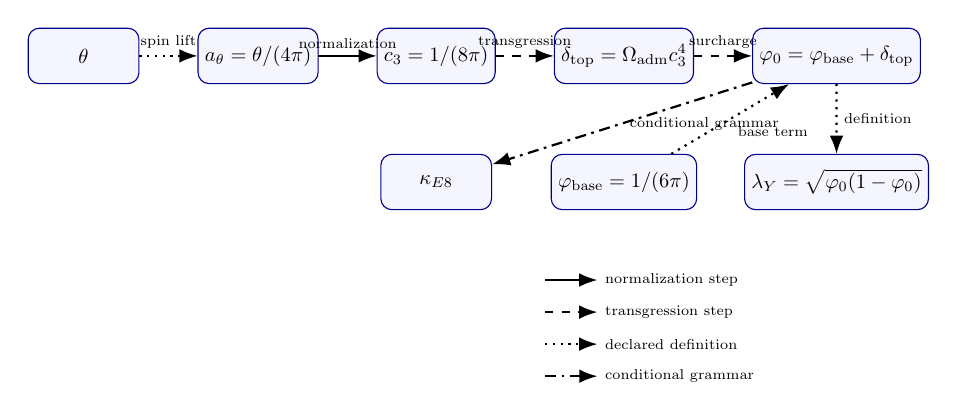
\begin{tikzpicture}[
    scale=0.74,
    transform shape,
    >=Latex,
    node distance=1.2cm and 1.0cm,
    box/.style={draw=blue!55!black, rounded corners, fill=blue!4, align=center, minimum width=1.9cm, minimum height=0.95cm},
    hardedge/.style={->, thick},
    bridgeedge/.style={->, dashed, thick},
    definedge/.style={->, dotted, thick},
    optedge/.style={->, dash pattern=on 4pt off 2pt on 1pt off 2pt, thick}
]
\node[box] (theta) {$\theta$};
\node[box, right=of theta] (a) {$\atheta=\theta/(4\pi)$};
\node[box, right=of a] (c3) {$\cthree=1/(8\pi)$};
\node[box, right=of c3] (delta) {$\deltatop=\Oadm \cthree^4$};
\node[box, right=of delta] (phi0) {$\phiz=\phibase+\deltatop$};
\node[box, below=of delta] (phibase) {$\phibase=1/(6\pi)$};
\node[box, below=of phi0] (lambda) {$\lambdaY=\sqrt{\phiz(1-\phiz)}$};
\node[box, below=of c3] (e8) {$\kappa_{E8}$};
\draw[definedge] (theta) -- node[above, font=\scriptsize] {spin lift} (a);
\draw[hardedge] (a) -- node[above, font=\scriptsize] {normalization} (c3);
\draw[bridgeedge] (c3) -- node[above, font=\scriptsize] {transgression} (delta);
\draw[definedge] (phibase) -- node[below right, font=\scriptsize] {base term} (phi0);
\draw[bridgeedge] (delta) -- node[above, font=\scriptsize] {surcharge} (phi0);
\draw[definedge] (phi0) -- node[right, font=\scriptsize] {definition} (lambda);
\draw[optedge] (phi0) -- node[right, font=\scriptsize] {conditional grammar} (e8);
\coordinate (legA) at ($(phibase.south west)+(-0.1,-1.2)$);
\draw[hardedge] (legA) -- ++(0.9,0) node[right, black, font=\scriptsize] {normalization step};
\coordinate (legB) at ($(legA)+(0,-0.55)$);
\draw[bridgeedge] (legB) -- ++(0.9,0) node[right, black, font=\scriptsize] {transgression step};
\coordinate (legC) at ($(legB)+(0,-0.55)$);
\draw[definedge] (legC) -- ++(0.9,0) node[right, black, font=\scriptsize] {declared definition};
\coordinate (legD) at ($(legC)+(0,-0.55)$);
\draw[optedge] (legD) -- ++(0.9,0) node[right, black, font=\scriptsize] {conditional grammar};
\end{tikzpicture}
\caption{Constant cascade used for technical bookkeeping, shown in the occupancy-reinterpretation form for $\deltatop$. Arrow styles encode algebraic role rather than claim status: normalization, transgression, declared definition, and conditional downstream grammar.}
\label{fig:constant-cascade}
\end{figure}

Here the arrow $\atheta\to\cthree$ records a normalization convention internal to the present setup, not an independently proved theorem beyond the declared seam and spin-lift normalization.

\begin{table}[t]
\centering
\scriptsize
\setlength{\tabcolsep}{3pt}
\begin{tabularx}{\linewidth}{@{}>{\raggedright\arraybackslash}p{0.10\linewidth}>{\raggedright\arraybackslash}p{0.18\linewidth}>{\raggedright\arraybackslash}p{0.12\linewidth}>{\raggedright\arraybackslash}p{0.11\linewidth}YY@{}}
\toprule
Symbol & Definition & Compiler role & First origin & Reappears in & Physical meaning \\
\midrule
$\theta$ & seam-loop angle & core datum & seam data & $\atheta$ & geometric rotation variable \\
$\atheta$ & $\theta/(4\pi)$ & hard normalization & spin lift & $\cthree$, phase grammar & normalized cover rotation \\
$\cthree$ & $1/(8\pi)$ & hard kernel constant & seam normalization & $\deltatop$, $\beta$, $\sigma$ & seam normalization constant \\
$\phibase$ & $1/(6\pi)$ & hard kernel constant & carrier geometry & $\phiz$ & base opening \\
$\deltatop$ & $\frac{3}{256\pi^4}$; bridge reading $\Oadm\cthree^4$ & hard kernel value with bridge occupancy reinterpretation & retained numerical kernel & $\phiz$, $\delta_2$ & topological surcharge \\
$\phiz$ & $\frac{1}{6\pi}+\frac{3}{256\pi^4}$ & hard corrected opening & retained numerical kernel & $\lambdaY$, $\beta$, flavor & minimal nontrivial opening \\
$\gamma$ & $\tr_EY^2=5/6$ & hard kernel invariant & carrier packet & $\kappa_{E8}$, $\delta_2$ & carrier norm \\
$B$ & $\rank E_3/\rank E_2=3/2$ & hard kernel invariant & carrier packet & $\delta_2$ & carrier rank ratio \\
$\Oadm$ & $3\times16=48$ & bridge quantity & family lift & $\deltatop$ & admissible chiral-state count \\
$\bone$ & $\frac43N_{\mathrm{fam}}+\frac1{10}N_\Phi$ & hard kernel output & abelian index & benchmark map & hypercharge trace coefficient \\
$\kappa_{E8}$ & $\gamma/\ln(248/60)$ & conditional grammar & Appendix~\ref{app:constants} & scale ladder & optional scale spacing \\
\bottomrule
\end{tabularx}
\caption{Constants atlas for the present manuscript.}
\label{tab:constants-atlas}
\end{table}

\subsection{\texorpdfstring{E$_8$}{E8} as downstream scale grammar}

In the present paper E$_8$ is not used as a primitive cause. The retained parameter is
\[
\kappa_{E8}:=\frac{\gamma}{\ln(248/60)}=\frac{5/6}{\ln(248/60)}.
\]
On the retained branch this means
\[
\begin{aligned}
\kappa_{E8}&\approx \num{0.58723},
&
f_a&\approx \num{8.86e10}\,\mathrm{GeV},
\\
m_a&\approx \num{65.19}\,\mu\mathrm{eV},
&
\nu_a&\approx \num{15.764}\,\mathrm{GHz}.
\end{aligned}
\]
The intended reading is a downstream scale grammar:
\begin{itemize}[leftmargin=1.5em, topsep=3pt, itemsep=2pt]
    \item the carrier packet fixes $\gamma=5/6$,
    \item $\kappa_{E8}$ then defines an optional ladder parameter,
    \item the ladder is allowed to organize scale spacing,
    \item but it does not replace the carrier theorem or the seam data.
\end{itemize}
In the fuller appendix-level grammar one may package a downstream block scale as
\[
X(n,r,I_1)=\frac{\Mplunred}{8}\,\sin^2\theta_{13}
\left(\frac{60-2n}{60}\right)^{\kappa_{E8}}
e^{-(8-r)/64}e^{-12\pi I_1},
\]
where $n$ is the ladder stage, $r$ a mild block-multiplicity label, and $I_1$ the dominant block trace. This makes the reading discipline explicit: the stage index orders the ladder, the trace controls most of the exponential suppression, and the extra block label only refines the scale. E$_8$ is therefore a downstream scale grammar, not a universal mass formula.

\subsection{Full stage atlas}

The full real-domain atlas up to $n=29$ extends the main-text robust table with restricted-scan candidates and IR tail conjectures. Rows are classified as \emph{robust} (restrictive grammar, unambiguous target), \emph{restricted-scan} (plausible but less constrained), or \emph{tail conjecture} (new trace class $I_1\in\{\frac{11}{12},\frac{7}{6}\}$ not yet derived from block structure).

\begin{table}[H]
\centering
\scriptsize
\setlength{\tabcolsep}{2pt}
\begin{tabularx}{\linewidth}{@{}>{\centering\arraybackslash}p{0.035\linewidth}>{\centering\arraybackslash}p{0.035\linewidth}>{\raggedright\arraybackslash}p{0.065\linewidth}>{\raggedleft\arraybackslash}p{0.12\linewidth}>{\raggedleft\arraybackslash}p{0.12\linewidth}>{\raggedright\arraybackslash}p{0.09\linewidth}>{\raggedright\arraybackslash}p{0.17\linewidth}Y@{}}
\toprule
$n$ & $r$ & $I_1$ & $X$ (GeV) & Target & Residual & Identification & Class \\
\midrule
$3$ & $8$ & $1/2$ & $\num{2.159e8}$ & $\num{2.160e8}$ & $0.06\%$ & $\mu_{\cthree}$ RG crossing & robust \\
$5$ & $5$ & $1/12$ & $\num{1.307e15}$ & $\num{1.31e15}$ & $0.2\%$ & seesaw $M_R$ & robust \\
$6$ & $6$ & $1$ & $\num{1.272}$ & $\num{1.27}$ & $0.2\%$ & charm band & restricted-scan \\
$8$ & $1$ & $17/16$ & $\num{0.1059}$ & $\num{0.10566}$ & $0.2\%$ & muon band & restricted-scan \\
$10$ & $1$ & $1/3$ & $\num{8.826e10}$ & direct search & --- & PQ scale $f_a$ & robust \\
$12$ & $2$ & $41/48$ & $\num{246.35}$ & $\num{246.22}$ & $0.05\%$ & EW vacuum $v$ & robust \\
$14$ & $4$ & $17/16$ & $\num{0.0921}$ & $\num{0.0927}$ & $0.6\%$ & pion band & robust \\
$15$ & $4$ & $1$ & $\num{0.935}$ & $\num{0.938}$ & $0.3\%$ & hadron anchor & robust \\
$21$ & $4$ & $1/6$ & $\num{3.051e13}$ & $\num{3.06e13}$ & $0.3\%$ & inflation $M$ & robust \\
$21$ & $5$ & $41/48$ & $\num{171.8}$ & $\num{172.6}$ & $0.4\%$ & top quark & robust \\
$24$ & $7$ & $5/8$ & $\num{7.895e5}$ & $\num{7.920e5}$ & $0.3\%$ & $\mu_{\phiz}$ RG crossing & robust \\
$25$ & $5$ & $1$ & $\num{0.498}$ & $\num{0.498}$ & $0.0\%$ & kaon band & robust \\
$25$ & $7$ & $41/48$ & $\num{125.5}$ & $\num{125.25}$ & $0.2\%$ & Higgs mass & robust \\
$26$ & $2$ & $1$ & $\num{0.417}$ & $\num{0.42}$ & $0.7\%$ & $\sqrt{\sigma}$ confinement & robust \\
$27$ & $6$ & $41/48$ & $\num{91.6}$ & $\num{91.19}$ & $0.4\%$ & $Z$ boson & restricted-scan \\
$28$ & $1$ & $7/6$ & $\num{5.105e-4}$ & $\num{5.110e-4}$ & $0.1\%$ & electron & tail conjecture \\
$29$ & $1$ & $11/12$ & $\num{4.210}$ & $\num{4.18}$ & $0.7\%$ & bottom quark & tail conjecture \\
\bottomrule
\end{tabularx}
\caption{Full E$_8$ stage atlas on the canonical branch up to the real-domain boundary $n=29$.}
\label{tab:e8-full-atlas}
\end{table}

\subsection{Compression identities on the minimal branch}

The main-text compression identities are developed in the dedicated section on compression identities and carrier exclusion. This appendix subsection collects additional arithmetic continuations and the compression chain summary.

\begin{remark}[Abelian package from occupancy and carrier norm]
On the canonical branch,
\[
\Oadm\gamma=48\cdot\frac56=40.
\]
Thus the characteristic coefficient $41$ is compressed to
\[
41=\Oadm\gamma+1=40+1,
\]
that is, fermionic occupancy trace plus one light Higgs doublet contribution.
Writing $b_Y:=5\bone/3$ for the usual hypercharge-normalized coefficient and using the block-index relation $k_B=\frac32 I_1(B)$ to define $I_1^{\mathrm{EW}}:=\frac{5}{24}\bone$ and $k_{\mathrm{EW}}:=\frac{5}{16}\bone$, one obtains the unified chain
\begin{equation}
\label{eq:41-chain}
48\,I_1^{\mathrm{EW}}
=32\,k_{\mathrm{EW}}
=10\,\bone
=\Oadm\gamma+1
=41.
\end{equation}
Equivalently,
\[
I_1^{\mathrm{EW}}=\frac{41}{48},
\qquad
k_{\mathrm{EW}}=\frac{41}{32},
\qquad
\bone=\frac{41}{10},
\qquad
b_Y=\frac{41}{6}.
\]
This is an algebraic signature rather than an accidental coincidence: the same integer $41$ appears simultaneously as electroweak block trace, E$_8$ exponent, UV hypercharge trace, and carrier occupancy times norm plus one.
\end{remark}

\begin{remark}[Rank lock and single-seed compression: main-text reference]
The rank-lock identity $2^{g-3}=g-1\Rightarrow g=5$ is proved as \Cref{prop:rank-lock} in the main text.
The single-seed compression and the Cabibbo inversion $\phiz=\frac12(1-\sqrt{1-4\lambda_C^2})$ with all derived inter-observable relations are given in \Cref{eq:cabibbo-inversion,eq:lambda-c-master}. The carrier exclusion theorems for wrong discrete worlds are in \Cref{thm:carrier-exclusion}.
\end{remark}

\subsection{Optional arithmetic continuations}

The next relations mix the main-text carrier with optional appendix-level E$_8$, inflation, or geometric notation. They are useful compression patterns, but their interpretation should remain conditional or conjectural.

\begin{remark}[60, 48, and \texorpdfstring{$5/4$}{5/4} on the optional ladder]
If the optional scale ladder is started at $D_1=60$, then
\[
\frac{D_1}{\Oadm}=\frac{60}{48}=\frac54=B\gamma.
\]
On the minimal branch one may also write the same number as
\[
\frac54=\frac{\gcar}{\gcar-1}\qquad (\gcar=5).
\]
This compresses the E$_8$ start index, the admissible chiral count, the mirror factor, and the two-defect coefficient to the same rational factor.
\end{remark}

\begin{remark}[Factorization of the two-defect coefficient]
From the main-text identity
\[
\delta_2=\frac54\,\deltatop^2
\qquad\text{and}\qquad
\deltatop=\Oadm\,\cthree^4
\]
one obtains
\[
\delta_2=2880\,\cthree^8.
\]
On the canonical branch this factor admits the exact arithmetic decompositions
\[
2880=\Dstart\,\Oadm=60\cdot48,
\qquad
2880=|R(E_8)|\,\dim\mathfrak g_{\SM}=240\cdot12.
\]
The arithmetic identity is exact; the interpretation of this coincidence is still appendix-level.
\end{remark}

\begin{conjecture}[E$_8$ root-count reading]
On the same optional branch,
\[
|R(E_8)|=248-8=240=5\cdot48=5\,\Oadm.
\]
This suggests that the E$_8$ root count may be read as a fivefold unfolding of the admissible chiral packet, although that interpretation is not used as a main-text theorem.
\end{conjecture}

\begin{remark}[Reactor seed of the optional scale ladder]
If one writes the optional ladder as
\[
\varphi_n=\phiz e^{-\gamma}\left(\frac{D_n}{D_1}\right)^{\kappa_{E8}},
\qquad
D_n=60-2n,
\]
then the start value is precisely the reactor-angle seed,
\[
\varphi_n=\sin^2\theta_{13}\left(\frac{D_n}{D_1}\right)^{\kappa_{E8}}.
\]
Thus the appendix-level ladder may be read as a discrete continuation of the same seed that controls $\theta_{13}$.
\end{remark}

\begin{remark}[Conditional inflation-side compression]
If one imports the v2.8 Starobinsky-side relations
\[
A_s=\frac{N^2}{24\pi^2}\left(\frac{M}{\Mpl}\right)^2,
\qquad
\frac{M}{\Mpl}=\sqrt{8\pi}\,\cthree^4,
\]
then on the minimal branch
\[
A_s=\frac{N^2}{3\pi}\cthree^8=\frac{N^2}{8640\pi}\,\delta_2,
\]
and also
\[
\frac{M}{\Mpl}=\frac{\sqrt{8\pi}}{\Oadm}\,\deltatop.
\]
This is recorded only as an appendix-level compression identity because inflation is outside the present main-text claim surface.
\end{remark}

\begin{remark}[Dyonic intercept and the $\alpha$ kernel]
From the dyonic appendix the local astrophysical $\beta$ function reads
\[
\beta_{\mathrm{BH}}(r)=\frac{Q_eQ_m}{256\pi^4 r^2}=\frac{\deltatop}{3}\frac{Q_eQ_m}{r^2}=16\cthree^4\frac{Q_eQ_m}{r^2}.
\]
This is a cross-link between the EHT intercept channel and the $\alpha$ kernel: the same topological coefficient $\deltatop=48\cthree^4$ that pushes $\alpha$ into the precision zone also controls the local dyonic $\beta$ function. The local and cosmological sectors are therefore not two loose motifs but the same coefficient in two projections.
\end{remark}

\begin{remark}[Conditional occupancy route to gravity]
If the relative Einstein term is of the form
\[
S_{\mathrm{EH}}^{\mathrm{rel}}
=
\frac{\chi^2}{192\pi^2}\tr_{\mathcal H_{\mathrm{ch}}}\mathbf 1
\int d^4x\sqrt{-g}\,R,
\]
and if the family bridge identifies
\[
\tr_{\mathcal H_{\mathrm{ch}}}\mathbf 1=\Oadm=48,
\]
then
\[
\Mpl^2=\frac{\chi_0^2}{2\pi^2}.
\]
This is the occupancy-to-gravity route alluded to in the main text.
\end{remark}

\begin{remark}[Compression chain]
The appendix-level compression pattern may therefore be summarized as
\[
Y \leftrightarrow \inv,
\qquad
\gamma=\frac56,
\qquad
B\gamma=\frac54,
\qquad
\frac{D_1}{\Oadm}=\frac54,
\qquad
|R(E_8)|=5\,\Oadm,
\]
\[
\bone=\frac{\Oadm\gamma+1}{10},
\qquad
\Omega_b+\beta_{\mathrm{rad}}=\phiz,
\qquad
A_s=\frac{N^2}{8640\pi}\,\delta_2
\quad
\text{(conditional v2.8 import)}.
\]
\end{remark}

\subsection{Conditional minimal-parameter picture}

The next package is stronger but also more conditional. It assumes that the carrier rank, family multiplicity, and seam normalization are all read as closed rather than only partially inherited.

\begin{principle}[Conditional minimal-parameter compression]
Assume the canonical branch
\[
\gcar:=\rank E=5,
\qquad
N_{\mathrm{fam}}=3,
\qquad
\cthree=\frac{1}{8\pi}.
\]
Then the numerical kernel may be rewritten almost entirely in terms of
\[
(\pi,\gcar,N_{\mathrm{fam}})=(\pi,5,3).
\]
Indeed, on this branch one has
\[
\gamma=\frac56=\frac{\gcar}{\gcar+1},
\qquad
\dim S^+=2^{\gcar-1},
\qquad
\Oadm=N_{\mathrm{fam}}2^{\gcar-1}=48,
\]
\[
\phibase=\frac{1-\gamma}{\pi}=\frac{1}{(\gcar+1)\pi},
\qquad
\deltatop=\Oadm\,\cthree^4,
\qquad
\delta_2=\Dstart\,\Oadm\,\cthree^8,
\]
with
\[
\Dstart=\gcar\,\dim\mathfrak g_{\SM}=5\cdot 12=60,
\qquad
\Oadm=(\gcar-1)\dim\mathfrak g_{\SM}=4\cdot 12=48.
\]
\end{principle}

\begin{remark}[Compressed dependency chain]
Under the same conditional closure, the appendix-level numerical chain reads
\[
(\widetilde M\to M,\Seam,\inv,\chi)
\Longrightarrow
E_3\oplus E_2
\Longrightarrow
Y \leftrightarrow \inv
\Longrightarrow
S(U(3)\times U(2))
\Longrightarrow
S^+,
\]
\[
\Longrightarrow
N_{\mathrm{fam}}=3
\Longrightarrow
\Oadm=48
\Longrightarrow
(\deltatop,\delta_2,\phiz)
\Longrightarrow
(\alpha,\lambda_C,\beta_{\mathrm{rad}},\Omega_b,\sin^2\theta_{13}),
\]
with the optional E$_8$, inflationary, and gravity-side sectors then read as downstream continuations of the same compressed core.
\end{remark}

\section{Relative APS and superconnection setup}
\label{app:aps}

The geometric completion uses APS-type relative data \cite{aps1975}. In practice this means:
\begin{itemize}[leftmargin=1.5em, topsep=3pt, itemsep=2pt]
    \item one works with a declared pair $(D,D_{\mathrm{ref}})$ rather than a single unanchored operator,
    \item boundary conditions on the seam $\Seam$ are part of the definition of the relative index,
    \item the $\eta$-term keeps track of the residual spectral asymmetry,
    \item the superconnection package is used in the same spirit as the spectral-action tradition \cite{chamseddineConnes1997}, but here always with an explicit reference subtraction.
\end{itemize}

The appendix is intentionally short. Its role is to make the common reference structure visible without pretending that the full heat-kernel computation has already been completed.

\section{Yukawa kernels and positivity lemmas}
\label{app:yukawa}

The transport program is based on the regularized kernel
\[
\mathcal Y_f^{(\varepsilon)}=(D_f^\dagger D_f+\varepsilon^2)^{-1}.
\]
Three remarks are important.
\begin{enumerate}[leftmargin=1.5em, topsep=3pt, itemsep=3pt]
    \item The regulator $\varepsilon$ is not optional: without it the kernel becomes ill-defined exactly where the admissibility question is most delicate.
    \item Positivity of the kernel is a transport-side selection principle, not yet a proved theorem of the hard kernel.
    \item Residual prefactors $\Lambda_{f,j}$ are bounded transport data that still require an operator-level closure. They must remain visible and must not be rhetorically hidden as if the entire mass map were already derived without remainder.
\end{enumerate}

\begin{remark}[Positive-kernel determinant route to strong CP]
If the physical mass map is written in the polar form
\[
M_f=U_{f,L}H_fU_{f,R}^\dagger,
\qquad
H_f>0,
\qquad
U_{f,L},U_{f,R}\in SU(3)_F,
\]
with $H_f$ induced by the positive transport kernel $\mathcal Y_f^{(\varepsilon)}$, then the induced determinant phase vanishes:
\[
\arg\det M_f=0.
\]
At the same time weak CP may survive through
\[
V_{\mathrm{CKM}}=U_{u,L}^\dagger U_{d,L}.
\]
Combined with the sheet-odd cancellation of $\theta_{\mathrm{sheet}}$ in the relative action, this is the algebraic core of the conditional strong-CP route summarized in the main text.
\end{remark}

\section{Optional record algebra, horizons, and prediction semantics}
\label{app:record}

This appendix keeps the record-level constructions available without letting them dominate the scope of explicit claims in the main paper.

\subsection{Minimal admissible vacuum}

At finite volume or with a declared cutoff, an admissible vacuum candidate is written as
\[
\rho_B
:=
\argmin_{\rho\in\Vadm}\tr(\rho\Hrel),
\]
provided the relative Hamiltonian is lower bounded on the admissible domain. In the absence of a full existence theorem this should be read as a minimizing-sequence statement, not as a solved cosmological theorem.

\subsection{Record growth principle}

The optional record algebra is
\[
\Arec(t):=\bigoplus_{\Delta_i>\Hhub(t)}\mathcal A_i,
\qquad
S_{\mathrm{rec}}(t)=\log\dim\Arec(t).
\]
As $\Hhub(t)$ decreases, more stable channels open. The intended arrow-of-time claim is therefore
\[
\frac{dS_{\mathrm{rec}}}{dt}>0,
\]
but only as a record-growth principle, not as a replacement for detailed nonequilibrium dynamics.

\subsection{Observer algebra and Born-type evaluation}

An observer is modeled as a stable pointer subalgebra
\[
\Aobs\subset\Arec.
\]
With orthogonal projectors $P_i\in\Aobs$ one writes the measurement channel
\[
\mathcal M_O(\rho)=\sum_i(P_i\rho P_i)\otimes |i\rangle\langle i|.
\]
In finite-dimensional sectors, positivity, additivity on orthogonal decompositions, and phase invariance lead to the standard Born-type assignment
\[
p_i=\tr(\rho P_i).
\]
The claim is therefore only a constrained evaluation principle on admissible sectors, not a new theorem about measurement in all settings.

\subsection{Horizons as conjectural inner seams}

If a horizon is modeled as an inner seam, the manuscript uses only an approximate factorization language,
\[
\mathcal H_{\mathrm{out}}\otimes\mathcal H_H\otimes\mathcal H_{\mathrm{in}},
\]
or, better, an algebraic split on an appropriate code subspace. This appendix intentionally avoids selling the factorization as exact fundamental structure.

\subsection{Prediction semantics}

The appendix-level prediction map is
\[
Q=(\rho_0,\mathcal O_Q,\Delta_Q,t,\mathcal C_Q,\mathcal R_Q),
\qquad
\Pred(Q)=\mathcal R_Q\!\left(\tr(\rho_tE_Q(\Delta)),\mathcal C_Q\right),
\]
with
\[
\rho_t=U(t)\rho_0U^\dagger(t).
\]
This is kept only as an optional formal extension.

\section{Extended benchmarks}
\label{app:benchmarks}

\subsection{Extended comparison rows and supplementary checks}

\begin{table}[H]
\centering
\scriptsize
\begin{tabularx}{\linewidth}{@{}>{\raggedright\arraybackslash}p{0.18\linewidth}>{\raggedleft\arraybackslash}p{0.17\linewidth}>{\raggedleft\arraybackslash}p{0.17\linewidth}>{\raggedright\arraybackslash}p{0.22\linewidth}>{\raggedright\arraybackslash}p{0.14\linewidth}@{}}
\toprule
Observable & TFPT value & Reference value & Role & Status \\
\midrule
$\delta_{\mathrm{CKM}}$ & \num{1.198} rad & \num{1.196} rad & unresolved transport comparison & appendix comparison row \\
$m_{\pi^0}$ & \num{134.979} MeV & \num{134.977} MeV & hadronic out-of-sample check & appendix comparison row \\
$m_{bb}$ & \num{0.0015} eV & $< \num{0.2}$ eV & neutrinoless double-beta interface & appendix interface \\
$\eta_B$ & \num{5.97e-10} & \num{6.13e-10} & leptogenesis-side interface & appendix interface \\
$m_a$ & \num{65.2} $\mu$eV & direct-search target & axion mass interface & appendix interface \\
$\nu_a$ & \num{15.76} GHz & direct-search band & haloscope target frequency & appendix interface \\
\bottomrule
\end{tabularx}
\caption{Extended comparison rows kept out of the main text.}
\label{tab:extended-benchmarks}
\end{table}

\subsection{Supplementary mass-source rows}

The compact main-text mass ledgers intentionally suppress explicit formula detail. The source rows collected here retain that information without forcing the main text to read like a mixed formula notebook.

\begin{table}[H]
\centering
\scriptsize
\begin{tabularx}{\linewidth}{@{}>{\raggedright\arraybackslash}p{0.10\linewidth}>{\raggedright\arraybackslash}p{0.46\linewidth}>{\raggedleft\arraybackslash}p{0.16\linewidth}Y@{}}
\toprule
Particle & TFPT formula or source row & TFPT value & Status note \\
\midrule
$e$ & $\tfrac{v}{\sqrt2}\,\tfrac{16\pi}{7}\phiz^5$ & \num{0.52096} MeV & constant-factory candidate \\
$\mu$ & $\tfrac{v}{\sqrt2}\,\tfrac{4\pi}{3}\phiz^3$ & \num{107.49} MeV & constant-factory candidate \\
$\tau$ & $\tfrac{v}{\sqrt2}\,\tfrac{7\pi}{6}\phiz^2$ & \num{1.7688} GeV & constant-factory candidate \\
$\nu_1$ & minimal normal-ordering branch & $0$ & oscillation-inversion branch \\
$\nu_2$ & $\sqrt{\Delta m_{21}^2}$ & \num{8.614e-3} eV & derived from oscillation inversion \\
$\nu_3$ & $\sqrt{\Delta m_{31}^2}$ with seesaw cross-check & \num{5.015e-2} eV & seesaw cross-check gives \num{4.616e-2} eV \\
$u$ & ChPT ratio inversion anchored to $m_s$ & \num{2.195} MeV & derived; $\overline{\mathrm{MS}}$ at $2$ GeV \\
$d$ & $m_s/(m_s/m_d)$ & \num{4.67} MeV & derived; $\overline{\mathrm{MS}}$ at $2$ GeV \\
$s$ & strange-quark anchor in the light-quark solver & \num{93.4} MeV & anchor-dependent; $\overline{\mathrm{MS}}$ at $2$ GeV \\
$c$ & up-type ratio ladder with $m_c/m_u=\num{486.92}$ & \num{1.27} GeV & threshold input fixes the absolute scale \\
$b$ & down-type ratio ladder with $m_b/m_s=\num{43.79}$ & \num{4.18} GeV & threshold input fixes the absolute scale \\
$t$ & up-type ratio ladder with $m_t/m_c=\num{133.01}$ & \num{172.57} GeV & pole / $\overline{\mathrm{MS}}$ distinction remains external \\
$\pi^0$ & GMOR relation from $(m_u+m_d)$ and $\langle\bar qq\rangle$ & \num{134.979} MeV & hadronic out-of-sample check \\
$p$ & hadron mass ladder & \num{935.03} MeV & derived hadronic scale check \\
\bottomrule
\end{tabularx}
\caption{Supplementary mass-source rows referenced by the compact main-text mass surface.}
\label{tab:mass-source-supplement}
\end{table}

For the main-text baryon-fraction comparison we use the Planck 2018 base-$\Lambda$CDM conversion
\[
\Omega_b=\frac{\Omega_b h^2}{h^2},
\qquad
h=\frac{H_0}{100},
\]
so the quoted $\Omega_b$ row is not a free-floating cosmology number but an explicit reconstruction from the Planck parameter pair $(\Omega_b h^2,H_0)$ adopted in the suite ledger.

\begin{thebibliography}{99}

\bibitem{aps1975}
M.~F.~Atiyah, V.~K.~Patodi, and I.~M.~Singer,
\newblock \emph{Spectral asymmetry and Riemannian geometry. I},
\newblock Math. Proc. Cambridge Philos. Soc. \textbf{77} (1975), 43--69.

\bibitem{chamseddineConnes1997}
A.~H.~Chamseddine and A.~Connes,
\newblock \emph{The spectral action principle},
\newblock Commun. Math. Phys. \textbf{186} (1997), 731--750.

\bibitem{codata2022}
P.~J.~Mohr, D.~B.~Newell, and B.~N.~Taylor,
\newblock \emph{CODATA recommended values of the fundamental physical constants: 2022 update},
\newblock NIST / CODATA reference set, \url{https://physics.nist.gov/cuu/Constants/}, accessed March 2026.

\bibitem{pdg2025}
S.~Navas et al.\ (Particle Data Group),
\newblock \emph{Review of Particle Physics},
\newblock Phys.\ Rev.\ D \textbf{110} (2024), 030001; 2025 online update, \url{https://pdg.lbl.gov/2025/}, accessed March 2026.

\bibitem{nufit2025}
NuFIT Collaboration,
\newblock \emph{NuFIT global analysis of neutrino oscillation data},
\newblock website snapshot based on data available through November 2025, \url{https://www.nu-fit.org/}, accessed March 2026.

\bibitem{planck2018}
Planck Collaboration,
\newblock \emph{Planck 2018 results. VI. Cosmological parameters},
\newblock Astron. Astrophys. \textbf{641} (2020), A6.

\bibitem{minamiKomatsu2020}
Y.~Minami and E.~Komatsu,
\newblock \emph{New extraction of the cosmic birefringence from the Planck 2018 polarization data},
\newblock Phys. Rev. Lett. \textbf{125} (2020), 221301.

\bibitem{eskilt2023}
J.~R.~Eskilt et al.,
\newblock \emph{Cosmoglobe DR1 results. II. Constraints on isotropic cosmic birefringence from reprocessed WMAP and Planck LFI data},
\newblock Astron. Astrophys. \textbf{679} (2023), A144.

\bibitem{sullivan2025}
R.~M.~Sullivan, A.~Abghari, P.~Diego-Palazuelos, L.~T.~Hergt, and D.~Scott,
\newblock \emph{Planck PR4 (NPIPE) map-space cosmic birefringence},
\newblock arXiv:2502.07654.

\end{thebibliography}

\end{document}
